\documentclass[class=report,crop=false]{standalone}
\usepackage[screen]{../exo7book}

\begin{document}

\definecolor{coul_prive}{rgb}{0.93,0.26,0}
\definecolor{coul_public}{rgb}{0.06,0.63,0}

%\newcommand{\prive}[1]{{\bf\color{coul_prive} #1}}
%\newcommand{\public}[1]{{\color{coul_public} #1}}
\newcommand{\prive}[1]{\relax\ifmmode{\color{coul_prive} #1}\else{\bf\color{coul_prive} #1}\fi}
\newcommand{\public}[1]{\relax\ifmmode{\color{coul_public} #1}\else{\bf\color{coul_public} #1}\fi}


%====================================================================
\chapitre{Cryptographie}
%====================================================================

\insertvideo{g8RmT-CwTMo}{partie 1. Le chiffrement de César}

\insertvideo{rUlqxHGKJ68}{partie 2. Le chiffrement de Vigenère}

\insertvideo{oGDPtm8pYPM}{partie 3. La machine Enigma et les clés secrètes}

\insertvideo{6KfJXl-Kvws}{partie 4. La cryptographie à clé publique}

\insertvideo{D4zFKzeARcg}{partie 5. L'arithmétique pour RSA}

\insertvideo{Xlal_d4zyfo}{partie 6. Le chiffrement RSA}

%%%%%%%%%%%%%%%%%%%%%%%%%%%%%%%%%%%%%%%%%%%%%%%%%%%%%%%%%%%%%%%%
\section{Le chiffrement de César}

%-------------------------------------------------------
\subsection{César a dit...}

Jules César a-t-il vraiment prononcé la célèbre phrase : \\
\centerline{\public{DOHD \  MDFWD \ HVW}}
ou bien comme le disent deux célèbres Gaulois : \og Ils sont fous ces romains ! \fg.

En fait César, pour ses communications importantes à son armée, cryptait ses messages.
Ce que l'on appelle le chiffrement de César est un décalage des lettres :
pour crypter un message, $\prive{A}$ devient $\public{D}$, $\prive{B}$ devient $\public{E}$,
$\prive{C}$ devient $\public{F}$,...

$$\prive{A} \longmapsto \public{D} \quad \prive{B} \longmapsto \public{E} \quad \prive{C} \longmapsto \public{F}
\quad   \ldots \qquad \prive{W} \longmapsto \public{Z} \quad
\prive{X} \longmapsto \public{A} \quad \prive{Y} \longmapsto \public{B} \quad \prive{Z} \longmapsto \public{C}$$

Voici une figure avec l'alphabet d'origine en haut et en \prive{rouge},
en correspondance avec l'alphabet pour le chiffrement en-dessous et en \public{vert}.


{\centering
            \includegraphics[width=0.8\textwidth]{figures/Cesar_plan_3.png}

}
Nous adopterons la convention suivante, en \public{vert} c'est la partie du message à laquelle
tout le monde a accès (ou qui pourrait être intercepté), c'est donc le message crypté.
Alors qu'en \prive{rouge} c'est la partie du message confidentiel,
c'est le message en clair.

Pour prendre en compte aussi les dernières lettres de l'alphabet, il est plus judicieux de représenté l'alphabet sur un anneau.
Ce décalage est un \defi{décalage circulaire} sur les lettres de l'alphabet.

{\centering
            \includegraphics[width=0.5\textwidth]{figures/Cesar_3.png}

}

Pour déchiffrer le message de César, il suffit de décaler les lettres dans l'autre sens,
$\public{D}$ se déchiffre en $\prive{A}$, $\public{E}$ en $\prive{B}$,...

Et la célèbre phrase de César est : \\
\centerline{\prive{ALEA \  JACTA \  EST}}
qui traduite du latin donne \og Les dés sont jetés \fg.


%-------------------------------------------------------
\subsection{Des chiffres et des lettres}

Il est plus facile de manipuler des nombres que des lettres, aussi nous passons à une formulation arithmétique.
Nous associons à chacune des $26$ lettres de $A$ à $Z$ un nombre de $0$ à $25$.
En termes mathématiques, nous définissons une bijection :
$$f : \big\{ A, B, C, \ldots, Z\big\} \longrightarrow \big\{ 0, 1, 2, \ldots, 25\big\}$$
par
$$A \longmapsto 0 \quad B \longmapsto 1 \quad C \longmapsto 2 \quad \ldots  \quad Z \longmapsto 25$$

Ainsi "\public{A L E A}" devient "\public{0 11 4 0}".

Le chiffrement de César est un cas particulier de \defi{substitution mono-alphabétique},
c'est-à-dire un chiffrement lettre à lettre.

Quel est l'intérêt ? Nous allons voir que le chiffrement de César correspond à une opération mathématique très simple.
Pour cela, rappelons la notion de congruence et l'ensemble $\Zz/26\Zz$.

%-------------------------------------------------------
\subsection{Modulo}


Soit $n \ge 2$ un entier fixé.
\begin{definition}
 On dit que \defi{$a$ est congru à $b$ modulo $n$},
si $n$ divise $b-a$. On note alors
$$a \equiv b \pmod n.$$
\end{definition}

%Remarque : on note aussi souvent $a \equiv b \pod n$.


Pour nous $n=26$. Ce qui fait que $28 \equiv  2 \pmod {26}$,
car $28-2$ est bien divisible par $26$. De même $85 = 3 \times 26+ 7$ donc
$85 \equiv  7 \pmod {26}$.

On note $\Zz/26 \Zz$ l'ensemble de tous les éléments de $\Zz$ modulo $26$. Cet ensemble peut par exemple être représenté par les $26$ éléments $\{0,1,2,\ldots, 25\}$. En effet, puisqu'on compte modulo $26$ :
$$0,\ 1,\ 2,\ \ldots,\  25, \quad \text{ puis } \quad  26\equiv 0,\  27 \equiv  1,\  28 \equiv  2,  \ldots,\quad  52\equiv 0,\  53\equiv 1, \ldots$$
et de même $-1\equiv 25$, $-2\equiv 24$,...

\bigskip


Plus généralement $\Zz / n \Zz$ contient $n$ éléments.
Pour un entier $a \in \Zz$ quelconque, son \defi{représentant}
dans $\{0,1,2,\ldots, n-1\}$ s'obtient comme le reste $k$
de la division euclidienne de $a$ par $n$ :
$a = bn + k$.
De sorte que $a \equiv  k \pmod n$ et $0 \le k < n$.


\bigskip


De façon naturelle l'addition et la multiplication d'entiers se transposent dans $\Zz/n\Zz$.

\bigskip

Pour $a,b \in \Zz/n\Zz$, on associe $a+b \in \Zz/n\Zz$.

Par exemple dans
$\Zz/26\Zz$, $15+13$ égale $2$. En effet
$15+13 = 28 \equiv 2 \pmod{26}$.
Autre exemple : que vaut $133+64$ ?
$133+64=197=7\times 26 +15 \equiv 15 \pmod {26}$.
Mais on pourrait procéder différemment :
tout d'abord $133 = 5 \times 26 + 3 \equiv 3 \pmod {26}$
et $64 = 2 \times 26 + 12 \equiv 12 \pmod{26}$.
Et maintenant sans calculs :
$133 + 64 \equiv 3 + 12 \equiv 15 \pmod{26}$.

\bigskip


On fait de même pour la multiplication :
pour $a,b \in \Zz/n\Zz$, on associe $a \times b \in \Zz/n\Zz$.

Par exemple $3 \times 12$ donne $10$ modulo $26$, car $3\times 12 = 36 = 1 \times 26 + 10 \equiv 10 \pmod{26}$.
De même : $3 \times 27 = 81 = 3 \times 26 + 3 \equiv 3 \pmod{26}$.
Une autre façon de voir la même opération est d'écrire d'abord
$27=1 \pmod{26}$ puis $3 \times 27 \equiv 3 \times 1 \equiv 3 \pmod{26}$.




%-------------------------------------------------------
\subsection{Chiffrer et déchiffrer}

Le chiffrement de César est simplement une addition dans $\Zz/26\Zz$ !
Fixons un entier $k$ qui est le décalage (par exemple $k=3$ dans
l'exemple de César ci-dessus) et définissons la \defi{fonction de chiffrement de César de décalage $k$}
qui va de l'ensemble $\Zz/26 \Zz$ dans lui-même :
\mybox{$C_k : \left\{\begin{array}{rcl}
    \Zz/26 \Zz  & \longrightarrow & \Zz/26 \Zz \\
                x     & \longmapsto & x{\color{red}+k} \\
  \end{array}\right.$}

Par exemple, pour $k=3$ : $C_3(0)=3$, $C_3(1)=4$\ldots

Pour déchiffrer, rien de plus simple ! Il suffit d'aller dans l'autre sens, c'est-à-dire ici de soustraire.
La \defi{fonction de déchiffrement de César de décalage $k$} est
\mybox{$D_k : \left\{\begin{array}{rcl}
    \Zz/26 \Zz  & \longrightarrow & \Zz/26 \Zz \\
                x     & \longmapsto &  x{\color{red}-k} \\
  \end{array}\right.$}

En effet, si $1$ a été chiffré en $4$, par la fonction $C_3$ alors $D_3(4)=4-3=1$.
On retrouve le nombre original.
Mathématiquement, $D_k$ est la bijection réciproque de $C_k$, ce qui implique que pour tout
$x \in \Zz/26 \Zz$ :
\mybox{$D_k \big( C_k(x) \big) = x$}
En d'autres termes, si $x$ est un nombre, on applique la fonction de chiffrement
pour obtenir le nombre crypté $y=C_k(x)$ ; ensuite
la fonction de déchiffrement fait bien ce que l'on attend d'elle
$D_k(y)=x$, on retrouve le nombre original $x$.

\begin{center}
\begin{tikzpicture}
  \coordinate (A) at (-1,0);
  \coordinate (B) at (1,0);
  \node[left] at (A) {$\Zz/26\Zz$};
  \node[right] at (B) {$\Zz/26\Zz$};
  \draw[->, blue, very thick] ($(A)+(0,0.25)$) to[bend left, thick]node[above, midway]{$C_k$} ($(B)+(0,0.25)$);
  \draw[->, blue, very thick] ($(B)+(0,-0.25)$) to[bend left, thick]node[below, midway]{$D_k$} ($(A)+(0,-0.25)$);
\end{tikzpicture}
\end{center}


Une autre façon de voir la fonction de déchiffrement est de remarquer que
$D_k(x)=C_{-k}(x)$. Par exemple $C_{-3}(x)=x+(-3) \equiv x+23 \pmod{26}$.


\bigskip


Voici le principe du chiffrement : Alice veut envoyer des messages secrets à Bruno.
Ils se sont d'abord mis d'accord sur une clé secrète $k$, par exemple $k=11$.
Alice veut envoyer le message "\prive{COUCOU}" à Bruno.
Elle transforme "\prive{COUCOU}" en "\prive{2 14 20 2 14 20}".
Elle applique la fonction de chiffrement $C_{11}(x)=x+11$ à chacun des nombres :
"\public{13 25 5 13 25 5}" ce qui correspond au mot crypté "\public{NZFNZF}".
Elle transmet le mot crypté à Bruno, qui selon le même principe
applique la fonction de déchiffrement $D_{11}(x)=x-11$.


\begin{center}
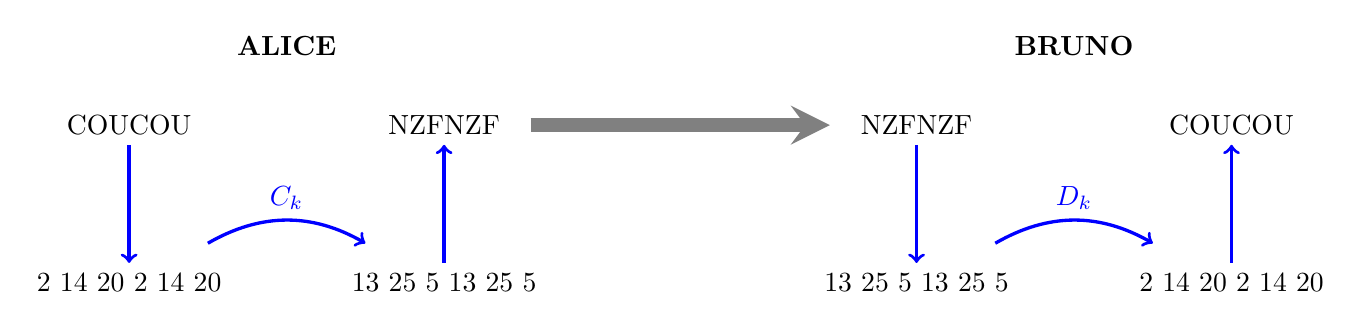
\begin{tikzpicture}

  \node at (-5,1) {\bf ALICE};
  \node at (5,1) {\bf BRUNO};
  \node at (-7,0) {\prive{COUCOU}};
  \node at (-7,-2) {\prive{2 14 20 2 14 20}};
  \node at (-3,-2) {\public{13 25 5 13 25 5}};
  \node at (-3,0) {\public{NZFNZF}};
  \node at (7,0) {\prive{COUCOU}};
  \node at (7,-2) {\prive{2 14 20 2 14 20}};
  \node at (3,-2) {\public{13 25 5 13 25 5}};
  \node at (3,0) {\public{NZFNZF}};

  \draw[->, blue, very thick] (-7,-0.25) to (-7,-1.75);
  \draw[<-, blue, very thick] (-3,-0.25) to (-3,-1.75);
  \draw[<-, blue, very thick] (7,-0.25) to (7,-1.75);
  \draw[->, blue, very thick] (3,-0.25) to (3,-1.75);

  \draw[->, blue, very thick] (-6,-1.5) to[bend left, thick]node[above, midway]{$C_k$} (-4,-1.5);
  \draw[<-, blue, very thick] (6,-1.5) to[bend right, thick]node[above, midway]{$D_k$} (4,-1.5);

  \draw[line width=5pt,>=stealth,->,gray] (-1.9,0) to (1.9,0);
\end{tikzpicture}
\end{center}



\bigskip


\begin{exemple}
Un exemple classique est le "rot13"  (pour rotation par un décalage de $13$) :
$$C_{13}(x) = x +13$$
et comme $-13 \equiv 13 \pmod{26}$ alors $D_{13}(x)=x+13$.
La fonction de déchiffrement est la même que la fonction de chiffrement !

Exemple : déchiffrez le mot "\public{PRFNE}".% ["CESAR"]

\end{exemple}




Notons ici deux points importants pour la suite :
tout d'abord nous avons naturellement considéré un mot comme une succession de lettres,
et chaque opération de chiffrement et déchiffrement s'effectue sur un bloc d'une seule lettre.
Ensuite nous avons vu que chiffrer un message est une opération mathématique
(certes sur un ensemble un peu spécial).


%-------------------------------------------------------
\subsection{Espace des clés et attaque}

Combien existe-t-il de possibilités de chiffrement par la méthode de César ?
Il y a $26$ fonctions $C_k$ différentes, $k=0,1,\ldots,25$. Encore une fois, $k$ appartient à
$\Zz / 26 \Zz$, car par exemple les fonctions $C_{29}$ et $C_3$ sont identiques.
Le décalage $k$ s'appelle la \defi{clé de chiffrement}, c'est l'information nécessaire
pour crypter le message. Il y a donc $26$ clés différentes et l'\defi{espace des clés} est
$\Zz/26\Zz$.


\bigskip

Il est clair que ce chiffrement de César est d'une sécurité très faible.
Si Alice envoie un message secret à Bruno et que Chloé intercepte ce message,
il sera facile pour Chloé de le décrypter même si elle ne connaît pas la clé secrète $k$.
L'attaque la plus simple pour Chloé est de tester ce que donne chacune des $26$ combinaisons
possibles et de reconnaître parmi ces combinaisons laquelle donne un message compréhensible.



%-------------------------------------------------------
\subsection{Algorithmes}


Les ordinateurs ont révolutionné la cryptographie et surtout
le décryptage d'un message intercepté.
Nous montrons ici, à l'aide du langage \Python\ comment programmer et attaquer
le chiffrement de César. Tout d'abord la fonction de chiffrement se programme en une seule ligne :

\insertcode{algos/cesar-tex1.py}{cesar.py (1)}

Ici \codeinline{x} est un nombre de $\{0,1,\ldots,25\}$ et \codeinline{k}
est le décalage. \codeinline{(x+k)\%26} a pour valeur le reste modulo $26$ de la somme \codeinline{(x+k)}.
Pour le décryptage, c'est aussi simple :

\insertcode{algos/cesar-tex2.py}{cesar.py (2)}


Pour chiffrer un mot ou une phrase, il n'y a pas de problèmes théoriques, mais seulement
des difficultés techniques :
\begin{itemize}
  \item Un mot ou une phrase est une chaîne de caractères, qui en fait se comporte comme une liste.
  Si \codeinline{mot} est une chaîne alors \codeinline{mot[0]} est la première lettre,
  \codeinline{mot[1]} la deuxième lettre... et
  la boucle \codeinline{for lettre in mot:} permet de parcourir chacune des lettres.

  \item Pour transformer une lettre en un nombre, on utilise le code Ascii qui à chaque caractère
  associe un nombre, \codeinline{ord(A)} vaut $65$, \codeinline{ord(B)} vaut $66$...
  Ainsi \codeinline{(ord(lettre) - 65)} renvoie le rang de la lettre entre $0$ et $25$ comme nous l'avons fixé dès le départ.

  \item La transformation inverse se fait par la fonction \codeinline{chr} : \codeinline{chr(65)} renvoie
  le caractère \codeinline{A}, \codeinline{chr(66)} renvoie \codeinline{B}...

  \item Pour ajouter une lettre à une liste, faites
  \codeinline{maliste.append(lettre)}. Enfin pour transformer une liste de caractères
  en une chaîne, faites \codeinline{"".join(maliste)}.
\end{itemize}

Ce qui donne :

\insertcode{algos/cesar-tex3.py}{cesar.py (3)}


Pour l'attaque on parcourt l'intégralité de l'espace des clés : $k$ varie de $0$ à $25$.
Noter que pour décrypter les messages on utilise ici simplement la fonction de César avec
la clé $-k$.

\insertcode{algos/cesar-tex4.py}{cesar.py (4)}





%%%%%%%%%%%%%%%%%%%%%%%%%%%%%%%%%%%%%%%%%%%%%%%%%%%%%%%%%%%%%%%%
\section{Le chiffrement de Vigenère}


%-------------------------------------------------------
\subsection{Substitution mono-alphabétique}

%.............................
\subsubsection{Principe}

Nous avons vu que le chiffrement de César présente une sécurité très faible,
la principale raison est que l'espace des clés est trop petit : il y a seulement $26$
clés possibles, et on peut attaquer un message chiffré en testant
toutes les clés à la main.

Au lieu de faire correspondre circulairement les lettres, on associe maintenant à chaque lettre une autre lettre
(sans ordre fixe ou règle générale).

Par exemple :

% \begin{center}
% \begin{tabular}{|c|}
% \hline
% A B C D E F G H I J K L M N O P Q R S T U V W X Y Z \\
% \hline
% F Q B M X I T E P A L W H S D O Z K V G R C N Y J U \\
% \hline
% \end{tabular}
% \end{center}



{\scriptsize
\begin{center}
\begin{tabular}{|*{26}{c|}}
\hline
\prive{A}&\prive{B}&\prive{C}&\prive{D}&\prive{E}&\prive{F}&\prive{G}&\prive{H}&\prive{I}&\prive{J}&\prive{K}&\prive{L}&\prive{M}&\prive{N}&\prive{O}&\prive{P}&\prive{Q}&\prive{R}&\prive{S}&\prive{T}&\prive{U}&\prive{V}&\prive{W}&\prive{X}&\prive{Y}&\prive{Z}\\
\hline
\public{F}&\public{Q}&\public{B}&\public{M}&\public{X}&\public{I}&\public{T}&\public{E}&\public{P}&\public{A}&\public{L}&\public{W}&\public{H}&\public{S}&\public{D}&\public{O}&\public{Z}&\public{K}&\public{V}&\public{G}&\public{R}&\public{C}&\public{N}&\public{Y}&\public{J}&\public{U}\\
\hline
\end{tabular}
\end{center}
}
\bigskip


Pour crypter le message \\
\centerline{\prive{ETRE \ OU \ NE \ PAS \ ETRE \ TELLE \ EST \ LA \ QUESTION}}
on regarde la correspondance et on remplace la lettre \prive{E} par la lettre \public{X},
puis la lettre \prive{T} par la lettre \public{G}, puis la lettre \prive{R} par la lettre \public{K}...

Le message crypté est alors : \\
\centerline{\public{XGKX \ DR \ SX \ OFV \ XGKX \ GXWWX \ XVG \ WF \ ZRXVGPDS}}
Pour le décrypter, en connaissant les substitutions, on fait l'opération inverse.

\bigskip

Avantage : nous allons voir que l'espace des clés est gigantesque
et qu'il n'est plus question d'énumérer toutes les possibilités.

Inconvénients : la clé à retenir est beaucoup plus longue, puisqu'il
faut partager la clé constituée des $26$ lettres "FQBMX...".
Mais surtout, nous allons voir que finalement ce protocole de chiffrement est assez simple à \og craquer \fg.

%.............................
\subsubsection{Espace des clés}

Mathématiquement, le choix d'une clé revient au choix d'une bijection de
l'ensemble $\big\{ A,B,\ldots,Z \big\}$ vers le même ensemble $\big\{ A,B,\ldots,Z \big\}$.
Il y a $26!$ choix possibles. En effet pour la lettre A de l'ensemble de départ, il y a
$26$ choix possibles (nous avions choisi F), pour B il reste $25$ choix possibles
(tout sauf F qui est déjà choisi), pour C il reste $24$ choix...
enfin pour Z il ne reste qu'une seule possibilité, la seule lettre non encore choisie.
Au final il y a : $26\times 25 \times 24 \times \cdots \times 2 \times 1$ soit $26!$ choix de clés.
Ce qui fait environ $4 \times 10^{26}$ clés. Il y a plus de clés différentes que de grains de sable
sur Terre ! Si un ordinateur pouvait tester $1$ milliard de clés par seconde, il lui faudrait alors
$12$ milliards d'années pour tout énumérer.


%.............................
\subsubsection{Attaque statistique}

La principale faiblesse du chiffrement mono-alphabétique est qu'une même lettre
est toujours chiffrée de la même façon. Par exemple, ici \prive{E} devient \public{X}.
Dans les textes longs, les lettres %de la langue française %, et ceci est vrai pour toutes les langues,
n'apparaissent pas avec la même fréquence. Ces fréquences varient suivant la langue utilisée. En français, les lettres les plus rencontrées sont dans l'ordre : \\
\centerline{\prive{E S A I N T R U L O D C P M V Q G F H B X J Y Z K W}}
avec les fréquences (souvent proches et dépendant de l'échantillon utilisé) :
\begin{center}
\begin{tabular}{|c|c|c|c|c|c|c|c|c|c|c|}
\hline
\prive{E}&\prive{S}&\prive{A}&\prive{I}&\prive{N}&\prive{T}&\prive{R}&\prive{U}&\prive{L}&\prive{O}&\prive{D}\\
\hline
%14.699\%&8.012\%&7.540\%&7.184\%&6.895\%&6.888\%&6.496\%&6.129\%&5.636\%&5.298\%&3.661\%\\
14.69\%&8.01\%&7.54\%&7.18\%&6.89\%&6.88\%&6.49\%&6.12\%&5.63\%&5.29\%&3.66\%\\
\hline
\end{tabular}
\end{center}

Voici la méthode d'attaque : dans le texte crypté, on cherche la lettre qui apparaît le plus,
et si le texte est assez long cela devrait être le chiffrement du \prive{E}, la lettre qui apparaît
ensuite dans l'étude des fréquences devrait être le chiffrement du \prive{S},
puis le chiffrement du \prive{A}... On obtient des morceaux de texte clair sous
la forme d'une texte à trous et il faut ensuite deviner les lettres manquantes.

\bigskip

Par exemple, déchiffrons la phrase : \\
\centerline{\public{LHLZ \  HFQ  \ BC HFFPZ \  WH \  YOUPFH  \ MUPZH}}
On compte les apparitions des lettres : \\
\centerline{\public{H} : 6 \quad \public{F} : 4 \quad \public{P} : 3 \quad \public{Z} : 3}
On suppose donc que le \public{H} crypte la lettre \prive{E}, le \public{F} la lettre \prive{S},
ce qui donne \\
\centerline{*\prive{E}** \ \prive{ES}* \ ** \ \prive{ESS}** \ *\prive{E} \ ***\prive{SE} \ ****\prive{E}}

D'après les statistiques \public{P} et \public{Z} devraient se décrypter en \prive{A} et \prive{I}
(ou \prive{I} et \prive{A}).
Le quatrième mot "\public{HFFPZ}", pour l'instant décrypté en "\prive{ESS}**", se complète donc en
"\prive{ESSAI}" ou "\prive{ESSIA}".
La première solution semble correcte ! Ainsi \public{P} crypte \prive{A}, et
\public{Z} crypte \prive{I}.
La phrase est maintenant : \\
\centerline{*\prive{E}*\prive{I} \  \prive{ES}* \  ** \  \prive{ESSAI} \  *\prive{E} \ ***\prive{ASE} \ **\prive{AIE}}
En réfléchissant un petit peu, on décrypte le message : \\
\centerline{\prive{CECI \ EST \ UN \ ESSAI \ DE \ PHRASE \ VRAIE}}



%-------------------------------------------------------
\subsection{Le chiffrement de Vigenère}


%.............................
\subsubsection{Blocs}

L'espace des clés du chiffrement mono-alphabétique est immense, mais le
fait qu'une lettre soit toujours cryptée de la même façon représente une trop grande faiblesse.
Le chiffrement de Vigenère remédie à ce problème.
On regroupe les lettres de notre texte par blocs, par exemple ici par blocs de longueur $4$ : \\
\centerline{\prive{CETTE \ PHRASE \  NE \ VEUT \ RIEN \ DIRE}}
devient \\
\centerline{\prive{CETT \ EPHR \ ASEN \ EVEU \ TRIE \ NDIR \ E}}
(les espaces sont purement indicatifs, dans la première phrase ils séparent les mots,
dans la seconde ils séparent les blocs).


Si $k$ est la longueur d'un bloc, alors on choisit une clé constituée de $k$ nombres de $0$ à $25$ :
$(n_1,n_2,\ldots,n_k)$. Le chiffrement consiste à effectuer un chiffrement de César,
dont le décalage dépend du rang de la lettre dans le bloc :
\begin{itemize}
  \item un décalage de $n_1$ pour la première lettre de chaque bloc,
  \item un décalage de $n_2$ pour la deuxième lettre de chaque bloc,
  \item ...
  \item un décalage de $n_k$ pour la $k$-ème et dernière lettre de chaque bloc.
\end{itemize}

\bigskip

Pour notre exemple, si on choisit comme clé $(3,1,5,2)$ alors
pour le premier bloc "\prive{CETT}" :
\begin{itemize}
  \item un décalage de $3$ pour \prive{C} donne \public{F},
  \item un décalage de $1$ pour \prive{E} donne \public{F},
  \item un décalage de $5$ pour le premier \prive{T} donne \public{Y},
  \item un décalage de $2$ pour le deuxième \prive{T} donne \public{V}.
\end{itemize}

Ainsi "\prive{CETT}" de vient "\public{FFYV}".
Vous remarquez que les deux lettres \prive{T} ne sont pas cryptées par la même lettre
et que les deux \public{F} ne cryptent pas la même lettre.
On continue ensuite avec le deuxième bloc...

%.............................
\subsubsection{Mathématiques}

L'élément de base n'est plus une lettre mais un \defi{bloc}, c'est-à-dire un regroupement de lettres.
La fonction de chiffrement associe à un bloc de longueur $k$, un autre bloc de longueur $k$,
ce qui donne en mathématisant les choses :
\mybox{$C_{n_1,n_2,\ldots,n_k} : \left\{\begin{array}{rcl}
\Zz/26\Zz \times \Zz/26\Zz \times \cdots \times \Zz/26\Zz
& \longrightarrow & \Zz/26\Zz \times \Zz/26\Zz \times \cdots \times \Zz/26\Zz \\
 (x_1,x_2,\ldots,x_k) & \longmapsto & (x_1+n_1,x_2+n_2,\ldots,x_k+n_k) \\
\end{array}\right.$}

Chacune des composantes de cette fonction est un chiffrement de César.
La fonction de déchiffrement est juste $C_{-n_1,-n_2,\ldots,-n_k}$.

%.............................
\subsubsection{Espace des clés et attaque}

Il y a $26^k$ choix possibles de clés, lorsque les blocs sont de longueur $k$.
Pour des blocs de longueur $k=4$ cela en donne déjà $456\;976$, et même si un ordinateur teste
toutes les combinaisons possibles sans problème, il n'est pas aisé de parcourir
cette liste pour trouver le message en clair, c'est-à-dire celui qui est compréhensible !

Il persiste tout de même une faiblesse du même ordre que celle rencontrée dans le chiffrement mono-alphabétique : la lettre \prive{A}
n'est pas toujours cryptée par la même lettre, mais si deux lettres \prive{A} sont situées à la même position dans deux blocs différents
(comme par exemple "\prive{ALPH \ ABET}") alors elles seront cryptées par la même lettre.

Une attaque possible est donc la suivante : on découpe notre message en plusieurs listes,
les premières lettres de chaque bloc, les deuxièmes lettres de chaque bloc...
et on fait une attaque statistique sur chacun de ces regroupements.
Ce type d'attaque n'est possible que si la taille des blocs
est petite devant la longueur du texte.

%-------------------------------------------------------
\subsection{Algorithmes}

Voici un petit algorithme qui calcule la fréquence de chaque lettre d'une phrase.

\insertcode{algos/statistiques-tex.py}{statistiques.py}


Et voici le chiffrement de Vigenère.

\insertcode{algos/vigenere-tex.py}{vigenere.py}

%%%%%%%%%%%%%%%%%%%%%%%%%%%%%%%%%%%%%%%%%%%%%%%%%%%%%%%%%%%%%%%%
\section{La machine Enigma et les clés secrètes}


%-------------------------------------------------------
\subsection{Un secret parfait}

L'inconvénient des chiffrements précédents est qu'une même lettre est régulièrement chiffrée de la même façon,
car la correspondance d'un alphabet à un ou plusieurs autres est fixée une fois pour toutes,
ce qui fait qu'une attaque statistique est toujours possible.
Nous allons voir qu'en changeant la correspondance à chaque lettre, il est possible de créer un chiffrement
parfait !

Expliquons d'abord le principe à l'aide d'une analogie :
j'ai choisi deux entiers $m$ et $c$ tels que $m+c=100$.
Que vaut $m$ ? C'est bien sûr impossible de répondre car il y a plusieurs possibilités :
$0+100$, $1+99$, $2+98$,...
Par contre, si je vous donne aussi $c$ alors vous trouvez $m$ immédiatement $m=100-c$.

\bigskip

Voici le principe du chiffrement :
Alice veut envoyer à Bruno le message secret \prive{$M$} suivant : \\
\centerline{\prive{ATTAQUE \ LE \ CHATEAU}}
Alice a d'abord choisi une clé secrète \prive{$C$} qu'elle a transmise à Bruno.
Cette clé secrète est de la même longueur que le message (les espaces ne comptent pas)
et composée d'entiers de $0$ à $25$,
tirés au hasard.
Par exemple \prive{$C$} : \\
\centerline{[4, 18, 2, 0, 21, 12, 18, 13, 7, 11, 23, 22, 19, 2, 16, 9]}

Elle crypte la première lettre par un décalage de César donné par le premier entier :
\prive{A} est décalé de $4$ lettres et devient donc \public{E}.
La seconde lettre est décalée du second entier : le premier \prive{T} devient \public{L}.
Le second \prive{T} est lui décalé de $2$ lettres, il devient \public{V}.
Le \prive{A} suivant est décalé de $0$ lettre, il reste \public{A}...
Alice obtient un message chiffré \public{$X$} qu'elle transmet à Bruno : \\
\centerline{\public{ELVALGW \ YL \ NEWMGQD}}
Pour le décrypter, Bruno, qui connaît la clé, n'a qu'à faire le décalage dans l'autre sens.

Notez que deux lettres identiques (par exemples les \prive{T})
n'ont aucune raison d'être cryptées de la même façon.
Par exemple, les \prive{T} du message initial sont cryptés dans l'ordre
par un \public{L}, un \public{V} et un \public{M}.


\bigskip

Formalisons un peu cette opération. On identifie $A$ avec $0$, $B$ avec $1$, ..., $Z$ avec $25$.
Alors le message crypté \public{$X$} est juste la "somme" du message \prive{$M$}
avec la clé secrète \prive{$C$},
la somme s'effectuant lettre à lettre, terme à terme, modulo $26$.

Notons cette opération $\prive{M} \oplus \prive{C} = \public{X}$.

\begin{center}
\begin{tabular}{cccccccccccccccccccc}
&&\prive{A}&\prive{T}&\prive{T}&\prive{A}&\prive{Q}&\prive{U}&\prive{E}& &\prive{L}&\prive{E}& &\prive{C}&\prive{H}&\prive{A}&\prive{T}&\prive{E}&\prive{A}&\prive{U}\\
&&\prive{0}&\prive{19}&\prive{19}&\prive{0}&\prive{16}&\prive{20}&\prive{4}& &\prive{11}&\prive{4}& &\prive{2}&\prive{7}&\prive{0}&\prive{19}&\prive{4}&\prive{0}&\prive{20}\\
\multicolumn{10}{l}{$\oplus$}\\
&&\prive{4}&\prive{18}&\prive{2}&\prive{0}&\prive{21}&\prive{12}&\prive{18}& &\prive{13}&\prive{7}& &\prive{11}&\prive{23}&\prive{22}&\prive{19}&\prive{2}&\prive{16}&\prive{9}\\
~\\
\hline
~\\
=&&\public{4}&\public{11}&\public{21}&\public{0}&\public{11}&\public{6}&\public{22}& &\public{24}&\public{11}& &\public{13}&\public{4}&\public{22}&\public{12}&\public{6}&\public{16}&\public{3}\\
&&\public{E}&\public{L}&\public{V}&\public{A}&\public{L}&\public{G}&\public{W}& &\public{Y}&\public{L}& &\public{N}&\public{E}&\public{W}&\public{M}&\public{G}&\public{Q}&\public{D}\\
\end{tabular}
\end{center}

Bruno reçoit \public{$X$} et connaît \prive{$C$}, il effectue donc $\public{X} \ominus \prive{C} = \prive{M}$.


Pourquoi ce système est-il inviolable ? Pour chacune des lettres, c'est exactement le même problème que trouver
$m$, sachant que $m+c=x$ (où $x=100$), mais sans connaître $c$. Toutes les possibilités
pour $m$ pourraient être juste. Et bien sûr, dès que l'on connaît $c$, la solution est triviale : $m=x-c$.

Il y a trois principes à respecter pour que ce système reste inviolable :
\begin{enumerate}
  \item La longueur de la clé est égale à la longueur du message.

  \item La clé est choisie au hasard.

  \item La clé ne sert qu'une seule fois.
\end{enumerate}

Ce système appelé "masque jetable" ou chiffrement de Vernam  est parfait en théorie, mais sa mise en \oe uvre n'est pas pratique du tout !
Tout d'abord il faut que la clé soit aussi longue que le message. Pour un message
court cela ne pose pas de problème, mais pour envoyer une image par exemple cela devient très lourd.
Ensuite, il faut trouver un moyen sûr d'envoyer la clé secrète à son interlocuteur
avant de lui faire parvenir le message. Et il faut recommencer cette opération à chaque message, ou
bien se mettre d'accord dès le départ sur un \defi{carnet de clés} : une longue liste
de clés secrètes.

Pour justifier que ce système est vraiment inviolable voici une expérience amusante :
Alice veut envoyer le message \prive{$M$} ="\prive{ATTAQUE \ LE \ CHATEAU}" à Bruno, elle choisit la clé secrète
\prive{$C$}=[4, 18, 2, 0,...] comme ci-dessus et obtient le message chiffré \public{$X$}="\public{ELVA}..." qu'elle transmet à Bruno.

Alice se fait kidnapper par Chloé, qui veut l'obliger à déchiffrer son message.
Heureusement, Alice a anticipé les soucis : elle a détruit le message \prive{$M$}, la clé secrète \prive{$C$}
et a créé un faux message $M'$ et une fausse clé secrète $C'$.
Alice fournit cette fausse clé secrète $C'$ à Chloé, qui déchiffre le message par l'opération
$\public{X} \ominus C'$ et elle trouve le message bien inoffensif $M'$ : \\
\centerline{RECETTE \ DE \ CUISINE}
Alice est innocentée !


Comment est-ce possible ? Alice avait au préalable préparé un message neutre $M'$ de même longueur que \prive{$M$}
et calculé la fausse clé secrète
$C' = \public{X} \ominus M'$. Chloé a obtenu (par la contrainte) \public{$X$} et $C'$, elle déchiffre le message ainsi
$$\public{X} \ominus C' = \public{X} \ominus (\public{X} \ominus M') = (\public{X} \ominus \public{X}) \oplus M' = M'$$
Chloé trouve donc le faux message.

Ici la fausse clé $C'$ est : \\
\centerline{[13, 7, 19, 22, 18, 13, 18, 21, 7, 11, 10, 14, 20, 24, 3, 25]}
La première lettre du message chiffré est un \public{E}, en reculant de
$13$ lettres dans l'alphabet, elle se déchiffre en \prive{R}...


%-------------------------------------------------------
\subsection{La machine Enigma}

Afin de s'approcher de ce protocole de chiffrement parfait, il faut trouver un moyen de générer facilement de longues clés, comme si elles avaient
été générées au hasard. Nous allons étudier deux exemples utilisés en pratique à la fin du siècle dernier, une méthode électro-mécanique :
la machine Enigma et une méthode numérique : le \textsc{des}.

La machine Enigma est une machine électro-mécanique qui ressemble à une machine à écrire.
Lorsque qu'une touche est enfoncée, des disques internes sont actionnés et le caractère crypté s'allume.
Cette machine, qui sert aussi au déchiffrement, était utilisée pour les communications de l'armée allemande durant la seconde guerre mondiale.
Ce que les
Allemands ne savaient pas, c'est que les services secrets polonais et britanniques avaient réussi
à percer les secrets de cette machine et étaient capables de déchiffrer les messages transmis par les allemands.
Ce long travail d'études et de recherches a nécessité tout le génie d'Alan Turing et l'invention de l’ancêtre de l'ordinateur.

{\centering
            \includegraphics[width=0.4\textwidth]{figures/Enigma_Machine.png}

}

Nous symbolisons l'élément de base de la machine Enigma par deux anneaux :
\begin{itemize}
  \item Un anneau extérieur contenant l'alphabet "\prive{ABCDE}..." symbolisant le clavier de saisie des messages. Cet anneau est fixe.

  \item Un anneau intérieur contenant un alphabet dans le désordre (sur la figure "\public{GWQRU}..."). Cet anneau est mobile et effectue une rotation à chaque touche tapée au clavier.
  Il représente la clé secrète.
\end{itemize}

Voici, dans ce cas, le processus de chiffrement du mot "\prive{BAC}", avec la clé de chiffrement "\prive{G}" :
\begin{enumerate}
  \item \textbf{Position initiale.} L'opérateur tourne l'anneau intérieur de sorte que le \prive{A} extérieur et fixe
  soit en face du \public{G} intérieur (et donc \prive{B} en face de \public{W}).

{\centering
            \includegraphics[width=0.4\textwidth]{figures/Enigma_0_bi_unesurune.png}

}

  \item  \textbf{Première lettre.} L'opérateur tape la première lettre du message : \prive{B}, la machine affiche la correspondance \public{W}.

  \item \textbf{Rotation.} L'anneau intérieur tourne de $1/26$ème de tour, maintenant le \prive{A} extérieur et fixe est en face du \public{W}, le \prive{B} en face du \public{Q},...

{\centering
            \includegraphics[width=0.4\textwidth]{figures/Enigma_1_bi_unesurune.png}

}

  \item \textbf{Deuxième lettre.} L'opérateur tape la deuxième lettre du message \prive{A}, la machine affiche la correspondance, c'est de nouveau
  \public{W}.

  \item \textbf{Rotation.} L'anneau intérieur tourne de $1/26$ème de tour, maintenant le \prive{A} extérieur et fixe est en face du \public{Q}, le \prive{B} en face du \public{R}, le \prive{C} en face du \public{U},...

{\centering
            \includegraphics[width=0.4\textwidth]{figures/Enigma_2_bi_unesurune.png}

}


   \item \textbf{Troisième lettre.} L'opérateur tape la troisième lettre du message \prive{C}, la machine affiche la correspondance \public{U}.

   \item \textbf{Rotation.} L'anneau intérieur  effectue sa rotation.

   \item \textbf{Message chiffré.} Le message crypté est donc "\public{WWU}"
\end{enumerate}

Cette méthode de chiffrement est identique à un chiffrement de type Vigenère pour une clé de longueur 26.
%Il n'y a pas d'attaque statistique possible, ici les deux W correspondent à des lettres différentes.
%Ce système est un \defi{chiffrement poly-alphabétique},
Il y a $26$ clés différents à disposition avec un seul anneau intérieur et identifiées par lettre de la position initiale : \prive{G}, \prive{W}, \prive{Q}... \prive{T} correspondant aux alphabets : "\prive{GWQ...PT}", "\prive{WQR...TG}", "\prive{QRU...GW}"...
%Un alphabet n'est utilisé que pour une lettre, puis on passe à l'alphabet suivant,...

En fait, la machine Enigma était beaucoup plus sophistiquée, il n'y avait pas un mais plusieurs anneaux intérieurs.
Par exemple pour deux anneaux intérieurs comme sur la figure : \prive{B} s'envoie sur {\bf\color{myorange}W}, qui s'envoie sur \public{A} ;
la lettre \prive{B} est cryptée en \public{A}.
Ensuite l'anneau intérieur numéro 1 effectue $1/26$ème de tour. La lettre  \prive{A} s'envoie sur {\bf\color{myorange}W}, qui s'envoie sur \public{A} ;
la lettre \prive{A} est cryptée en \public{A}.
Lorsque l'anneau intérieur numéro 1 a fait une rotation complète ($26$ lettres ont été tapées) alors l'anneau intérieur numéro 2 effectue $1/26$ème
de tour. C'est comme sur un compteur kilométrique, lorsque le chiffre des kilomètres parcourt $0,1,2,3,...,9$,
alors au kilomètre suivant, le chiffre des kilomètres est $0$ et celui des dizaines de kilomètres
est augmenté d'une unité.

{\centering
            \includegraphics[width=0.4\textwidth]{figures/Enigma_0_bi_unesurdeux.png}
            \qquad
            \includegraphics[width=0.4\textwidth]{figures/Enigma_0_tri_deuxsurdeux.png}

}

S'il y a trois anneaux, lorsque l'anneau intérieur 2 a fait une rotation complète, l'anneau intérieur 3 tourne de $1/26$ème
de tour. Il y a alors $26^3$ clés différentes facilement identifiables par les trois lettres des positions initiales des anneaux.

Il fallait donc pour utiliser cette machine, d'abord choisir les disques (nos anneaux intérieurs) les placer dans un certain ordre,
fixer la position initiale de chaque disque. Ce système était rendu largement plus complexe avec l'ajout de correspondances par fichage entre les lettres du clavier (voir photo). Le nombre de clés possibles dépassait plusieurs milliards de milliards !

~

{\centering
            \includegraphics[width=0.4\textwidth]{figures/Enigma-plugboard.jpg}

}



%
% %-------------------------------------------------------
% \subsection{Des zéros et des uns}
%
% Les ordinateurs ont révolutionné la cryptographie, car il est devenu possible d'effectuer des recherches
% exhaustives sur des milliards de possibilités. Les cryptographes doivent aussi apprendre le langage des ordinateurs
% qui ne connaissent que deux nombres : $0$ et $1$.
%
% Les deux seuls nombres sont $0$ et $1$, l'addition est celle de $\Zz/2\Zz$ :
% $$0+0=0 \qquad 0+1=1 \qquad 1+0=1 \qquad \color{red}{1+1=0}$$
%
% Si on a deux mots $m$ et $c$ composés de $0$ et de $1$ alors on peut définir l'addition
% $m \oplus c$, cette addition se fait \emph{bit} par \emph{bit} (c'est-à-dire colonne par colonne, sans retenue).
%
% Exemple $m = 10101010$, $c = 01110011$, notons $x= m \oplus c$ :
% $$\begin{array}{lccccccccc}
% m \quad &        & 1&0&1&0&1&0&1&0 \\
% c & \oplus & 0&1&1&1&0&0&1&1 \\
% \hline
% x &        & 1&1&0&1&1&0&0&1 \\
% \end{array}$$
% Ainsi la somme est $x=11011001$ (attention : cela ne correspond pas à l'addition des nombres
% en écriture binaire, ici $1+1=0$).
%
%
% Pour nous, $m$ est le message en clair, $c$ la clé de chiffrement et $x$ le message crypté.
% Comment déchiffrer le message ? Connaissant $x$ et $c$, c'est très facile.
% Comme $1+1=0$, alors $-1=+1$ donc ajouter ou soustraire est la même opération !
% Pour décrypter le message, il suffit donc de calculer $x\oplus c$ et on retrouve $m$.
% On peut aussi le prouver de la façon suivante : comme $0+0=0$ et $1+1=0$ alors
% quelque soit $c$, $c \oplus c=0$. Donc
% $$x \oplus c = (m \oplus c) \oplus c = m \oplus (c \oplus c) = m \oplus 0 = m.$$
% %Vérifiez-le sur l'exemple ci-dessus.
%


%-------------------------------------------------------
\subsection{La ronde des chiffres : DES}

La machine Enigma génère mécaniquement un alphabet différent à chaque caractère crypté, tentant de se rapprocher d'un chiffrement parfait.
Nous allons voir une autre méthode, cette fois numérique : le DES. Le DES
(\emph{Data Encryption Standard}) est un protocole de chiffrement par blocs.
Il a été, entre 1977 et 2001, le standard de chiffrement pour les organisations
du gouvernement des États-Unis et par extension pour un grand nombre de pays dans le monde.

\bigskip

Commençons par rappeler que l'objectif est de générer une clé aléatoire
de grande longueur. Pour ne pas avoir à retenir l'intégralité de cette
longue clé, on va la générer de façon pseudo-aléatoire à partir d'une petite clé.

Voyons un exemple élémentaire de suite pseudo-aléatoire.
% Nous donnons ci-après un exemple très simple de génération de clés secondaires.
% Les clés produites sont construites à l'aide d'opérations mathématiques à
% partir d'une clé principale, on ne peut donc pas parler de génération aléatoire,
% on parlera de génération pseudo-aléatoire.

Soit $(u_n)$ la suite définie par la donnée de $(a,b)$ et de $u_0$
et la relation de récurrence
$$u_{n+1} \equiv a\times u_n + b \pmod{26}.$$
%$(a,b)$ et $u_0$ est la clé courte et la suite des $(u_n)_{n\in\Nn}$
%nous servirait de clé longue.
Par exemple pour $a=2$, $b=5$ et $u_0=6$, alors les premiers termes de la suites sont :
$$6 \quad 17\quad 13\quad 5\quad 15 \quad9\quad 23\quad 25\quad 3 \quad11\quad 1 \quad7\quad 19\quad 17\quad 13\quad 5$$

Les trois nombres $(a,b,u_0)$ représentent la clé principale et la suite des $(u_n)_{n\in\Nn}$ les clés secondaires.

Avantages : à partir d'une clé principale courte (ici trois nombres) on a généré une longue liste de clés secondaires.
Inconvénients : la liste n'est pas si aléatoire que cela, elle se répète ici avec une période de longueur $12$ : $17, 13, 5,..., 17, 13, 5,...$


\bigskip

%Commençons par rappeler que l'objectif est de générer une clé aléatoire de grande longueur. Pour ne pas avoir à retenir l'intégralité de cette longue clé, on va la générer de façon pseudo-aléatoire à partir d'une petite clé.


%\bigskip
Le système DES est une version sophistiquée de ce processus :
à partir d'une clé courte et d'opérations élémentaires on crypte un message.
Comme lors de l'étude de la machine Enigma, nous allons présenter une
version très simplifiée de ce protocole afin d'en expliquer les étapes élémentaires.

%Le système DES est une version sophistiquée de ce processus :
%à partir d'une clé courte et d'opérations élémentaires on crypte un message. Voyons son principe sur un modèle très simplifié.


Pour changer, nous allons travailler modulo $10$.
Lorsque l'on travaille par blocs, les additions se font \emph{bit} par \emph{bit}. Par exemple :
$[1 \ 2 \ 3 \  4] \oplus [7\  8\  9\  0] = [8\  0\  2\  4]$ car ($1+7 \equiv 8 \pmod{10}$,
$2+8\equiv 0 \pmod{10}$,...)

Notre message est coupé en blocs, pour nos explications ce seront des blocs de longueur $8$. La clé est de longueur $4$.

Voici le message (un seul bloc): $M = [1\  2\  3\  4\  5\  6\  7\  8]$ et voici la clé : $C=[3\  1\  3\  2]$.

\bigskip

\textbf{\'Etape 0. Initialisation.}
On note $M_0=M$ et on découpe $M$ en une partie gauche et une partie droite
$$M_0 = [ G_0 \ \|\  D_0] = [1\  2\  3\  4\  \| \ 5\  6\  7\  8]$$

\bigskip

\textbf{\'Etape 1. Premier tour.}
On pose
$$M_1 = [ D_0 \ \|\  C \oplus \sigma(G_0)]$$
où $\sigma$ est une permutation circulaire.

On effectue donc trois opérations pour passer de $M_0$ à $M_1$ :
\begin{enumerate}
  \item On échange la partie droite et la partie gauche de $M_0$ :
$$M_0  \longmapsto  [5\  6\  7\  8\  \|\  1\  2\  3\  4]$$
  \item Sur la nouvelle partie droite, on permute circulairement les nombres :
$$\longmapsto  [5\  6\  7\  8\  \|\ 2\  3\  4\  1]$$

  \item Puis on ajoute la clé secrète $C$ à droite (ici $C=[3\  1\  3\  2]$) :
$$\longmapsto  [5\  6\  7\  8\  \| \ 5\  4\  7\  3] = M_1$$
\end{enumerate}


\bigskip

On va recommencer le même processus. Cela revient à appliquer la formule de récurrence,
qui partant de $M_i=[G_i \ \| \ D_i]$, définit
$$M_{i+1} = [ D_i \ \| \ C \oplus \sigma(G_i)]$$

\textbf{\'Etape 2. Deuxième tour.}
On part de $M_1 = [5\  6\  7\  8\  \|\ 5\  4\  7\  3]$.
\begin{enumerate}
  \item On échange la partie droite et la partie gauche de $M_0$ :
$$M_0  \longmapsto  [5\  4\  7\  3\  \| \ 5\  6\  7\  8]$$
  \item Sur la nouvelle partie droite, on permute circulairement les nombres.
$$\longmapsto  [5\  4\  7\  3\  \| \ 6\  7\  8\  5]$$

  \item Puis on ajoute la clé secrète $C$ à droite.
$$\longmapsto  [5\  4\  7\  3\  \| \ 9\  8\  1\  7] = M_2$$
\end{enumerate}

On peut décider de s'arrêter après ce tour et renvoyer
le message crypté $X=M_2 = [5\  4\  7\  3\ 9\  8\  1\  7]$.

Comme chaque opération élémentaire est inversible,
on applique un protocole inverse pour déchiffrer.


Dans le vrai protocole du DES, les blocs sont de taille $64$ \emph{bits},
il y a plus de manipulations sur le message et les étapes mentionnées ci-dessus
sont effectuées $16$ fois (on parle de tours).
\`A chaque tour, une clé différente est utilisée.
Il existe donc un préambule à ce protocole :
générer $16$ clés secondaires (de longueur $48$ \emph{bits}) à partir de la clé principale, ce qui se fait
selon le principe de la suite pseudo-aléatoire $(u_n)$ expliquée plus haut.



%
% %-------------------------------------------------------
% \subsection{La ronde des chiffres : DES}
%
% Le DES (Data Encryption Standard) est un protocole de chiffrement par blocs.
% Il a été, entre 1977 et 2001, le standard de chiffrement pour les organisations
% du gouvernement des États-Unis et par extension d'un grand nombre de pays dans le monde.
%
% Le principe en est le suivant : après une phase d'initialisation,
% le message initial est "mélangé" à la clé de chiffrement et ce 16 fois de suite
% avant de subir une dernière transformation avant d'obtenir le message chiffré.
%
% Avant d'étudier sur un exemple une version simplifiée, formalisons ce protocole.
% L'alphabet utilisé est le plus simple possible, il s'agit de $\{0,1\}$. Il conviendra donc avant la mise en place d'avoir à disposition les outils permettant de transformer un texte en suite de bits regroupés par blocs.
% Le message initial noté $M$ aura une longueur de $2n$ et la clé de chiffrement une longueur $2k$ (nous préciserons $n$ et $k$ plus tard. \`A partir de la clé $K$, sont produites $d$ clés $K_1$, $K_2$... $K_d$. Le protocole est doté de certains outils spécifiques et notamment d'une application $f : \{0,1\}^{n+k}\longrightarrow \{0,1\}^{n}$ que nous expliciterons ci-après. Le schéma est le suivant : à partir de $I(M)=(G_0,D_0)$, c'est-à-dire l'image du message initial par une application $I$ de $\{0,1\}^{2n}\longrightarrow \{0,1\}^{2n}$ (de réciproque $I^{-1}$) que l'on découpe en deux parties de longueurs égales $n$ (gauche et droite), nous définissons une suite $(G_i,D_i)$ pour $1\leq i \leq d$ par :
% $$\left\{
% \begin{array}{rcl}
% G_i&=&D_{i-1}\\
% D_i&=&G_{i-1}\oplus f(K_i,D_{i-1})
% \end{array}
% \right.
% $$
% l'opération $\oplus$ étant définie comme dans le paragraphe précédent. Le texte chiffré est alors $C=I^{-1}(G_d,D_d)$.
%
% Comme tous les protocoles vus jusqu'ici, le protocole de déchiffrement associé est simple, il ne nécessite pas d'outils supplémentaires. En effet, il suffit de parcourir en sens inverse les étapes du chiffrement. En partant du message chiffré que nous noterons $(G_d,D_d)$, par récurrence pour $i$ variant de $d$ à $1$ :
% $$\left\{
% \begin{array}{rcl}
% D_{i-1}&=&L_{i}\\
% G_{i-1}&=&L_{i}\oplus f(K_i,G_{i})
% \end{array}
% \right.
% $$
% nous obtenons le message initial par $(G_0,D_0)$.
%
% Attardons nous maintenant aux fonctions $f$ :
% $$
% f(K,N)=PC(S(E(R)\oplus T))
% $$
% où
% \begin{itemize}
% \item $E$ est une application de $\{0,1\}^{n}$ dans $ \{0,1\}^{ef}$ ($e$ et $f$ entiers) et comme nous allons faire la somme $E(R)\oplus T$ où $T$ sera une clé $K_i$, ceci implique que les clés forgées à partir de la clé $K$ sont de longueur $ef$ ;
% \item $S$ est une transformation de  $\{0,1\}^{ef}$ dans $ \{0,1\}^{n}$ qui découpe les $ef$ bits en $e$ blocs de $f$ bits et qui transforme chaque bloc $B=(b_1,b_2...b_f)$ par ce qu'on appelle une $S$-boîte (il y en a donc $e$) ;
% \item chaque $S$-boîte est un tableau de $2^2$ lignes et $2^{f-2}$ colonnes contenant une élément de $2^{f-2}$ ; l'image d'un élément $B=(b_1b_2...b_f)$ est déterminé par le contenu de la ligne numérotée $(b_1b_f)$ et de la colonne dont numérotée $(b_2b_3...b_{f-1})$ ;
% \item $PC$ est un décalage à gauche (c'est-à-dire en général pour $l$ entier : $PC(b_1...b_l)=(b_2b_3...b_lb_1)$).
% \end{itemize}
%
% Il nous reste à expliquer la génération des clés $K_1$, $K_2$... $K_d$ de longueur $ef$ à partir de la clé $K$ de longueur $2k$. \`A l'image de ce qui est dit plus haut pour le chiffrement, le point de départ est $C1(K)=(KG_0,KD_0)$, c'est-à-dire l'image de la clé par une application $C1$ de $\{0,1\}^{2k}\longrightarrow \{0,1\}^{2k}$ que l'on découpe en deux parties de longueurs égales $k$ (gauche et droite). Nous définissons ensuite pour $i$ variant de $1$ à $d$ :
% $$\left\{
% \begin{array}{rcl}
% KG_i&=&PC^{v_i}(KG_{i-1})\\
% KD_i&=&PC^{v_i}(KD_{i-1})\\
% K_i&=&C2(KG_i,KD_i)
% \end{array}
% \right.
% $$
% où
% \begin{itemize}
% \item les $v_i$ ($1\leq i \leq d$) sont des entiers ;
% \item $C2$ est une application de $\{0,1\}^{2k}\longrightarrow \{0,1\}^{ef}$.
% \end{itemize}
%
% Afin de prendre en main ce protocole de chiffrement, nous allons en présenter sur un exemple une version simplifié proposée en 1997 par
% E. Schaefer.
%
% Voici tout d'abord la taille des objets manipulés :
% \begin{itemize}
% \item le message initial est de longueur $2n=8$,
% \item la clé est de longueur $2k=10$,
% \item les clés forgées sont de longueur $ef=8$,
% \item les $e=2$ $S$-boîtes possèdent $2^2=4$ lignes et $2^{f-2}=4$ colonnes,
% \item le nombre de tours effectués est $d=2$.
% \end{itemize}
%
% Ensuite les éléments constitutifs du protocole :
% \begin{itemize}
% \item $I : \{0,1\}^{8}\longrightarrow \{0,1\}^{8}$ défini par $I(a_1,a_2,a_3,a_4,a_5,a_6,a_7,a_8)=(a_2,a_6,a_3,a_1,a_4,a_8,a_5,a_7)$ ;
% \item $I^{-1} : \{0,1\}^{8}\longrightarrow \{0,1\}^{8}$ défini par $I(a_1,a_2,a_3,a_4,a_5,a_6,a_7,a_8)=(a_4,a_1,a_3,a_5,a_7,a_2,a_8,a_6)$ ;
% \item $E : \{0,1\}^{4}\longrightarrow \{0,1\}^{8}$ défini par $E(a_1,a_2,a_3,a_4)=(a_4,a_1,a_2,a_3,a_2,a_3,a_4,a_1)$ ;
% \item Les $S$-boîtes $S_0$ et $S_1$ à $4$ lignes et $4$ colonnes :
% $$
% S_0 : \begin{array}{c|c|c|c|c}
% &(0,0)&(0,1)&(1,0)&(1,1)\\
% \hline
% (0,0)&(0,1)&(0,0)&(1,1)&(1,0)\\
% \hline
% (0,1)&(1,1)&(1,0)&(0,1)&(0,0)\\
% \hline
% (1,0)&(0,0)&(1,0)&(0,1)&(1,1)\\
% \hline
% (1,1)&(1,1)&(0,1)&(1,1)&(1,0)\\
% \end{array}
% \qquad
% S_1 : \begin{array}{c|c|c|c|c}
% &(0,0)&(0,1)&(1,0)&(1,1)\\
% \hline
% (0,0)&(0,0)&(0,1)&(1,0)&(1,0)\\
% \hline
% (0,1)&(1,0)&(0,0)&(0,1)&(1,1)\\
% \hline
% (1,0)&(1,1)&(0,0)&(0,1)&(0,0)\\
% \hline
% (1,1)&(1,0)&(0,1)&(0,0)&(1,1)\\
% \end{array}
% $$
%
% \item $C1 : \{0,1\}^{10}\longrightarrow \{0,1\}^{10}$ défini par $E(a_1,a_2,a_3,a_4,a_5,a_6,a_7,a_8,a_9,a_{10})=(a_3,a_5,a_2,a_7,a_4,a_{10},a_1,a_9,a_8,a_6)$ ;
% \item $v_1=1$, $v_2=2$ ;
% \item $PC : \{0,1\}^{4}\longrightarrow \{0,1\}^{4}$ défini par $E(a_1,a_2,a_3,a_4)=(a_2,a_3,a_4,a_1)$ ;
% \item $C2 : \{0,1\}^{8}\longrightarrow \{0,1\}^{8}$ défini par $E(a_1,a_2,a_3,a_4,a_5,a_6,a_7,a_8)=(a_6,a_3,a_7,a_4,a_8,a_5,a_{10},a_9)$ ;
% \end{itemize}
%
% Nous détaillons maintenant les étapes pour les paramètres suivants :
% \begin{itemize}
% \item le texte initial de longueur 8 : $(0,1,1,0,1,0,0,1)$,
% \item la clé de chiffrement de longueur 10 : $(1,0,0,0,1,1,0,1,0,1)$.
% \end{itemize}
%
% \begin{enumerate}
% \item {\bf Préparation des clés}
%
%       \`A l'aide de la clé de chiffrement nous allons construire deux clés (la longueur de la données $v$ est 2) dont nous nous servirons dans la phase suivante.
%       \begin{itemize}
%       \item La clé subit la permutation $C1$ et est coupée en deux morceaux de longueur 4 : $C_0$ et $C_1$ :
%       $$C1(1,0,0,0,1,1,0,1,1,1)=(0, 1, 0, 0, 0,1, 1, 0, 1, 1) \quad \Longrightarrow \quad
%       KG_0=(0, 1, 0, 0, 0),  \quad KD_0=(1, 1, 0, 1, 1)$$
%       \item Première clé :
%       \begin{itemize}
%       \item Calcul de $KG_1=PC^{v_1}(KG_0)=PC^1(KG_0)$ et $KD_1=PC^1(KD_0)$ :
%       $$KG_1=(1, 0, 0, 0, 0), \qquad KD_1=(1, 0, 1, 1, 1).$$
%       \item Calcul de $K_1=C2(KG_1,KD_1)$ :
%       $$K_1=C2(1, 0, 0, 0, 0,1, 0, 1, 1, 1)=(1, 0, 0, 0, 1, 0, 1, 1).$$
%       \item Calcul de $KG_2=PC^{v_2}(KG_1)=PC^2(KG_1)$ et $KD_2=PC^2(KD_1)$ :
%       $$KG_2=(0, 0, 0, 1, 0),  \qquad KD_2=(1, 1, 1, 1, 0).$$
%       \item Calcul de $K_2=C2(KG_2,KD_2)$ :
%       $$K_2=C2(0, 0, 0, 1, 0,1, 1, 1, 1, 0)=(1, 0, 1, 1, 1, 0, 0, 1).$$
%       \end{itemize}
%       \end{itemize}
% \item {\bf Initialisation}
%
%       Préparation du texte initial : les bits du message initial sont permutées par $I$ :
%       $$I(0,1,1,0,1,0,0,1)=(1, 0, 1, 0, 0, 1, 1, 0) \quad \Longrightarrow \quad
%       G_0=(1, 0, 1, 0),  \quad D_0=(1, 0, 0, 1)$$
% \item {\bf Tours}
%
%       \begin{itemize}
%       %%%%%%%%%%%%%%%%%%%
%       \item Premier tour :
%       $$\begin{array}{rcl}
%       D_1&=&G_0\oplus f(K_1,D_0)\\
%       &=&G_0\oplus PC(S(E(D_0)\oplus K_1))\\
%       &=&G_0\oplus PC(S(E(0, 1, 1, 0)\oplus K_1))\\
%       &=&G_0\oplus PC(S((1, 1, 0, 0, 0, 0, 1, 1)\oplus (1, 0, 0, 0, 1, 0, 1, 1)))\\
%       &=&G_0\oplus PC(S(0, 1, 1, 0, 0, 1, 1, 1))
%       \end{array}$$
%       Nous devons trouver l'image par $S_0$ de $(0, 1, 1, 0)$, c'est-à-dire l'élément de la ligne $(0,0)$ et de la colonne  $(1,1)$ : $(1,0)$ et l'image par $S_1$ de $(0, 1, 1, 1)$, c'est-à-dire l'élément de la ligne $(0,1)$ et de la colonne  $(1,1)$ : $(1,1)$. D'où :
%       $$\begin{array}{rcl}
%       D_1&=&G_0\oplus PC(1,0,1,1)\\
%       &=&(1, 0, 1, 0)\oplus (0, 1, 1, 1) \\
%       &=&(1, 1, 0, 1)
%       \end{array}$$
%       Enfin :
%       $$G_1=(1, 0, 0, 1),  \quad D_1=(1, 1, 0, 1)$$
%       %%%%%%%%%%%%%%%%%%%
%       \item Second tour :
%       $$\begin{array}{rcl}
%       D_2&=&G_1\oplus f(K_2,D_1)\\
%       &=&G_1\oplus PC(S(E(D_1)\oplus K_2))\\
%       &=&G_1\oplus PC(S(E(1, 1, 0, 1)\oplus K_2))\\
%       &=&G_1\oplus PC(S((1, 1, 1, 0, 1, 0, 1, 1)\oplus (1, 0, 1, 1, 1, 0, 0, 1)))\\
%       &=&G_1\oplus PC(S(1, 0, 1, 0, 1, 0, 0, 0))
%       \end{array}$$
%       Nous devons trouver l'image par $S_0$ de $(1, 0, 1, 0)$, c'est-à-dire l'élément de la ligne $(1,0)$ et de la colonne  $(0,1)$ : $(1,0)$ et l'image par $S_1$ de $(1, 0, 0, 0)$, c'est-à-dire l'élément de la ligne $(1,0)$ et de la colonne  $(0,0)$ : $(1,1)$. D'où :
%       $$\begin{array}{rcl}
%       D_2&=&G_1\oplus PC(1,0,1,1)\\
%       &=&(1, 0, 0, 1)\oplus (0,1,1,1)\\
%       &=&(1, 1, 1, 0)
%       \end{array}$$
%       Enfin :
%       $$G_2=(1, 1, 1, 0),  \quad D_2=(1, 1, 0, 1)$$
%       \end{itemize}
%
% \item {\bf Finalisation}
%
%       Le message chiffré est alors $I^{-1}(G_2,D_2)=I^{-1}(1, 1, 1, 0, 1, 1, 0, 1)=(0,1,1,1,0,1,1,1)$.
%
%
% \end{enumerate}
%
% Pour conclure sur ce protocole, mentionnons les tailles des objets manipulés par le DES :
% \begin{itemize}
% \item le message initial est de longueur $2n=64$,
% \item la clé est de longueur $2k=64$,
% \item les clés forgées sont de longueur $ef=48$,
% \item les $e=8$ $S$-boîtes possèdent $2^2=4$ lignes et $2^{f-2}=16$ colonnes,
% \item le nombre de tours effectués est $d=16$.
% \end{itemize}
%


%%%%%%%%%%%%%%%%%%%%%%%%%%%%%%%%%%%%%%%%%%%%%%%%%%%%%%%%%%%%%%
\section{La cryptographie à clé publique}


Les Grecs pour envoyer des messages secrets rasaient la tête du messager,
tatouaient le message sur son crâne et attendaient que les cheveux repoussent
avant d'envoyer le messager effectuer sa mission !

Il est clair que ce principe repose uniquement sur le secret de la méthode.

%-------------------------------------------------------
\subsection{Le principe de Kerckhoffs}

Cette méthode rudimentaire va à l'encontre du principe de Kerckhoffs.
Le principe de Kerckhoffs s’énonce ainsi : \\
\centerline{<<La sécurité d'un système de chiffrement ne doit reposer que sur le secret de la clé.>>}

\medskip

Cela se résume aussi par : \\
\centerline{<<L'ennemi peut avoir connaissance du système de chiffrement.>>}

\bigskip

Voici le texte original d'Auguste Kerckhoffs de 1883
<<La cryptographie militaire>> paru dans le {\sl Journal des sciences militaires}.

Il traite notamment des enjeux de sécurité lors des correspondances :
\begin{quotation}
\sl
<<Il faut distinguer entre un système d'écriture chiffré, imaginé
pour un échange momentané de lettres entre quelques personnes
isolées, et une méthode de cryptographie destinée à régler pour
un temps illimité la correspondance des différents chefs d'armée entre eux.>>
\end{quotation}


Le principe fondamental est le suivant :
\begin{quotation}
\sl
<<Dans le second cas, [\ldots]
il faut que {\bf le système n'exige pas le secret},
et qu'il puisse sans inconvénient tomber entre les mains de
l'ennemi.>>
\end{quotation}
Ce principe est novateur dans la mesure
où intuitivement il semble opportun de dissimuler le maximum
de choses possibles : clé et système de chiffrement utilisés.
Mais l'objectif visé par Kerckhoffs est plus académique,
il pense qu'un système dépendant d'un secret mais dont
le mécanisme est connu de tous sera testé, attaqué, étudié,
et finalement utilisé s'il s'avère intéressant et robuste.

% \begin{quotation}
% \sl
% <<
% Si l'Administration veut mettre à profit tous les services
% que peut rendre un système de correspondance cryptographique
% bien combiné, elle doit absolument {\bf renoncer aux méthodes secrètes},
% et établir en principe qu'elle n'acceptera qu'un
% {\bf procédé qui puisse être enseigné} au grand jour dans
% nos écoles militaires, que nos élèves seront libres de communiquer à qui leur plaira.>>
% \end{quotation}

% Il est inutile de dire que ce principe n'a pas toujours
% été appliqué par la suite tant le sur plan des échanges
% militaires ou administratifs que sur le plan des échanges privés (entreprises ou personnes).

%-------------------------------------------------------
\subsection{Factorisations des entiers}

Quels outils mathématiques répondent au principe de Kerckoffs ?
%
% En effet, existe-t-il des fonctions qui même connues ne
% dévoilent pas toute leur subtilité ?

Un premier exemple est la toute simple multiplication !
En effet si je vous demande combien font $5\times7$, vous répondez $35$.
Si je vous demande de factoriser $35$ vous répondez $5\times 7$.
Cependant ces deux questions ne sont pas du même ordre de difficulté.
Si je vous demande de factoriser $1591$, vous aller devoir faire plusieurs tentatives,
alors que si je vous avais directement demandé de calculer $37\times 43$ cela ne pose
pas de problème.

Pour des entiers de plusieurs
centaines de chiffres le problème de factorisation ne peut être résolu
en un temps raisonnable, même pour un ordinateur.
C'est ce problème asymétrique qui est à la base de la cryptographie RSA
(que nous détaillerons plus tard) : connaître $p$ et $q$ apporte plus d'information utilisable
que $p\times q$. Même si en théorie à partir de $p\times q$ on peut retrouver $p$ et $q$,
en pratique ce sera impossible.

\bigskip

Formalisons ceci avec la notion de complexité.
La \defi{complexité} est le temps de calculs (ou le nombre d'opérations élémentaires)
nécessaire pour effectuer une opération.

Commençons par la complexité de l'addition :
disons que calculer la somme de deux chiffres (par exemple $6+8$) soit de complexité $1$
(par exemple $1$ seconde pour un humain, $1$ milliseconde pour un ordinateur).
Pour calculer la somme de deux entiers à $n$ chiffres, la complexité est d'ordre $n$
(exemple : $1234+2323$, il faut faire $4$ additions de chiffres,
donc environ $4$ secondes pour un humain).

La multiplication de deux entiers à $n$ chiffres est de complexité d'ordre $n^2$.
Par exemple pour multiplier $1234$ par $2323$ il faut faire
$16$ multiplications de chiffres (chaque chiffre de $1234$ est à multiplier par chaque chiffre
de $2323$).

Par contre la meilleure méthode de factorisation connue est de complexité d'ordre
$\exp(4n^\frac13)$ (c'est moins que $\exp(n)$, mais plus que $n^d$ pour tout $d$,
lorsque $n$ tend vers $+\infty$).

Voici un tableau pour avoir une idée de la difficulté croissante pour multiplier
et factoriser des nombres à $n$ chiffres :
\begin{center}
\begin{tabular}{|c|c|c|}
\hline
$n$ & multiplication & factorisation \\
\hline
\hline
3 & 9 & 320 \\
4 & 16 & 572 \\
5 & 25 & 934 \\
10 & 100 & 5\;528 \\
50 & 2\;500 & 2\;510\;835 \\
100 & 10\;000 & 115\;681\;968 \\
200 & 40\;000 & 14\;423\;748\;780 \\
\hline
\end{tabular}
\end{center}


%
% En effet, si quelqu'un vous donne un entier et vous affirme
% qu'il est produit de deux nombres premiers, saurez-vous
% trouver ces deux entiers ? Pour de petites valeurs, le
% problème semble accessible. Muni d'une calculatrice ou
% d'un ordinateur, vous pouvez vous attaquer à des problèmes
% de plus grande taille. Mais pour des entiers de plusieurs
% centaines de chiffres... le problème ne peut être résolu
% en un temps raisonnable. Ce problème très simple, il peut
% être compris par des enfants, est en fait redoutable
% lorsque la taille des objets, ici des entiers, grandit.
%
% Il existe plusieurs méthodes pour factoriser un entier,
% mais même les plus évoluées demandent des temps de calculs
% énormes. La complexité de la factorisation n'est pas
% polynomiale en la taille de l'entier dont on cherche la
% factorisation, elle est exponentielle ou sous-exponentielle.

%-------------------------------------------------------
\subsection{Fonctions à sens unique}

% Il existe bien d'autres outils mathématiques répondant à ces objectifs.
% Par exemple pour le stockage des mots de passe dans nos ordinateurs :
% les mots de passe ne sont généralement pas sauvegardés sur nos disques
% durs mais ce sont seulement leurs "empreintes". Au cours
% d'une authentification, le mot de passe que nous tapons au clavier
% subit une transformation et le résultat est comparé à ce qui est
% stocké sur la machine.

% La transformation utilisée est une
% \defi{fonction à sens unique}, le calcul de l'empreinte est possible,
% mais, connaissant l'empreinte, retrouver le mot de passe est impossible.

Il existe bien d'autres situations mathématiques asymétriques :
les \defi{fonctions à sens unique}.
En d'autres termes, étant donnée une fonction $f$, il est possible
connaissant $x$ de calculer <<facilement>> $f(x)$ ; mais connaissant
un élément de l'ensemble image de $f$, il est <<difficile>> ou impossible
de trouver son antécédent.

% Les termes "facile" et "difficile" n'ont
% pas de définition bien précise. On pourrait parler de calcul raisonnables
% ou déraisonnables en temps humain. En effet, s'il vous faut plusieurs
% siècles pour calculer un inverse, le caractère mathématique de la question
% est : je peux calculer l'inverse, mais en pratique cet inverse reste inatteignable.

Dans le cadre de la cryptographie, posséder une fonction à sens
unique qui joue le rôle de chiffrement n'a que peu de sens.
En effet, il est indispensable de trouver un moyen efficace afin de pouvoir déchiffrer les messages
chiffrés. On parle alors de \defi{fonction à sens unique avec trappe secrète}.

\bigskip

Prenons par exemple le cas de la fonction $f$ suivante : $$f : x \longmapsto x^3 \pmod{100}.$$
  \begin{itemize}
    \item Connaissant $x$, trouver $y=f(x)$ est facile, cela nécessite deux multiplications et deux divisions.
    \item Connaissant $y$ image par $f$ d'un élément $x$ ($y=f(x)$), retrouver $x$ est difficile.
  \end{itemize}


\bigskip

Tentons de résoudre le problème suivant : trouver $x$ tel que $x^3 \equiv 11 \pmod{100}$.

On peut pour cela :

  \begin{itemize}
  \item soit faire une recherche exhaustive, c'est-à-dire essayer successivement
  $1$, $2$, $3$, ...,  $99$, on trouve alors :
    $$
    71^3=357\;911 \equiv 11 \pmod{100},
    $$
  \item soit utiliser la trappe secrète : $y \longmapsto y^7 \pmod{100}$ qui
  fournit directement le résultat !
    $$
    11^7= 19\;487\;171 \equiv 71 \pmod{100}.
    $$
  \end{itemize}

La morale est la suivante : le problème est dur à résoudre, sauf pour ceux qui
connaissent la trappe secrète. (Attention, dans le cas de cet exemple,
la fonction $f$ n'est pas bijective.)

%-------------------------------------------------------
\subsection{Chiffrement à clé secrète}

Petit retour en arrière.
Les protocoles étudiés dans les chapitres précédents étaient des \defi{chiffrements à clé secrète}.
De façon imagée, tout se passe
comme si Bruno pouvaient déposer son message dans un coffre fort pour Alice,
Alice et Bruno étant les seuls à posséder la clé du coffre.
\begin{center}
\begin{tikzpicture}
  \node at (-0.7,0){
  \includegraphics[height=3cm]{figures/coffre.png}
  };
  \node at (-3,-3) {\bf ALICE};
  \node at (-5,-1) {\bf BRUNO};

  \draw[->, blue, ultra thick] (-5,-0.7) to[bend left, thick]node[above, midway]{} (-1,0);
  \draw[->, blue, ultra thick] (-1.2,-0.5) to[bend right, thick]node[above, midway]{} (-3,-2.7);

\end{tikzpicture}
\end{center}

En effet, jusqu'ici, les deux interlocuteurs se partageaient une même clé qui servait
à chiffrer (et déchiffrer) les messages.
Cela pose bien sûr un problème majeur : Alice et Bruno doivent d'abord se communiquer la clé.
\begin{center}
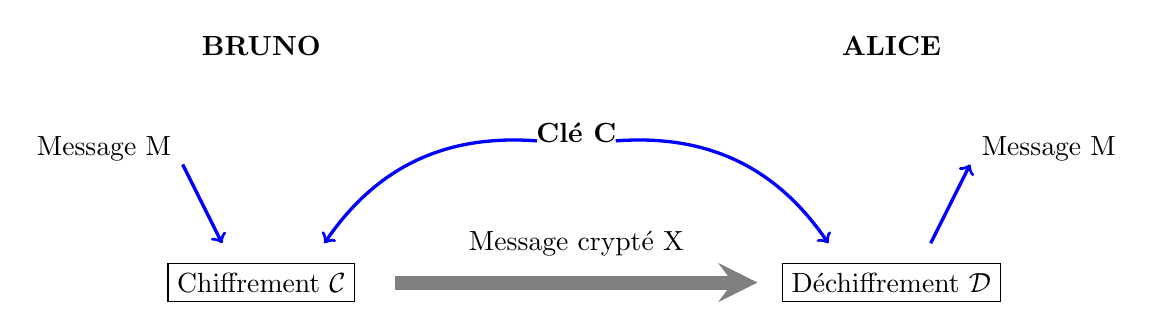
\begin{tikzpicture}

  \node at (4,3) {\bf ALICE};
  \node at (-4,3) {\bf BRUNO};

  \draw[line width=5pt,>=stealth,->,gray] (-2.3,0) to (2.3,0);

  \node at (-6,1.7) {\prive{Message M}};
  \node at (6,1.7) {\prive{Message M}};
  \node at (0,0.5) {\public{Message crypté X}};
  \node at (0,1.9) {\bf Clé C};
  \draw (-4,0)node[draw]{Chiffrement \public{$\mathcal{C}$}};
  \draw (4,0)node[draw]{Déchiffrement \public{$\mathcal{D}$}};

  \draw[->, blue, very thick] (-0.5,1.8) to[bend right, thick] (-3.2,0.5);
  \draw[->, blue, very thick] (0.5,1.8) to[bend left, thick] (3.2,0.5);

  \draw[->, blue, very thick] (-5,1.5) to (-4.5,0.5);
  \draw[<-, blue, very thick] (5,1.5) to (4.5,0.5);
\end{tikzpicture}
\end{center}

% \begin{figure}[htbp]
%   \begin{center}
%     \setlength{\unitlength}{2547sp}%
%     \begin{picture}(5700,2235)(2101,-3961)
%       \thinlines
%         \put(3301,-3961){\makebox(0,0)[cb]{Bruno}}
%         \put(6601,-3961){\makebox(0,0)[cb]{Alice}}
%         \put(3301,-2061){\makebox(0,0)[cb]{\prive{$K$}}}
%         \put(6601,-2061){\makebox(0,0)[cb]{\prive{$K$}}}
%         \put(2101,-3061){\makebox(0,0)[cc]{\prive{$m$}}}
%         \put(3001,-3361){\framebox(600,600){\public{$C$}}}
%         \put(2401,-3061){\vector( 1, 0){600}}
%         \put(3301,-2161){\vector( 0,-1){600}}
%         \put(4801,-2761){\makebox(0,0)[cb]{\public{$c$}}}
%         \put(3601,-3061){\vector( 1, 0){2700}}
%         \put(6301,-3361){\framebox(600,600){\public{$D$}}}
%         \put(6901,-3061){\vector( 1, 0){600}}
%         \put(6601,-2161){\vector( 0,-1){600}}
%         \put(7801,-3061){\makebox(0,0)[cc]{\prive{$m$}}}
%         \put(4500,-3361){\includegraphics[height=1cm]{figures/coffre.jpg}}
%     \end{picture}
%   \end{center}
% \end{figure}


%-------------------------------------------------------
\subsection{Chiffrement à clé publique}

Les fonctions à sens unique à trappe donnent naissance
à des protocoles de chiffrement à clé publique.
L'association <<clé>> et <<publique>> peut paraître incongrue,
mais il signifie que le principe de chiffrement est accessible à tous mais
que le déchiffrement nécessite une clé qu'il faut bien sûr garder secrète.

\begin{center}
\begin{tikzpicture}
  \node at (-0.45,-0.56){
  \includegraphics[height=3cm]{figures/boite.png}
  };
  \node at (-3,-3) {\bf ALICE};
  \node at (-5,-1) {\bf BRUNO};

  \draw[->, myred, ultra thick] (-5,-0.7) to[bend left, thick]node[above, midway]{} (-1.5,-0.15);
  \draw[->, myred, ultra thick] (-2,-0.7) to[bend right, thick]node[above, midway]{} (-3,-2.7);

\end{tikzpicture}
\end{center}

De façon imagée, si Bruno veut envoyer un message à Alice,
il dépose son message dans la boîte aux lettres d'Alice, seule Alice pourra ouvrir sa boîte
et consulter le message. Ici la clé publique est symbolisée par la boîte aux lettre, tout le monde peut y déposer
un message, la clé qui ouvre la boîte aux lettres est la clé privée d'Alice, que Alice doit conserver
à l'abri.

\begin{center}
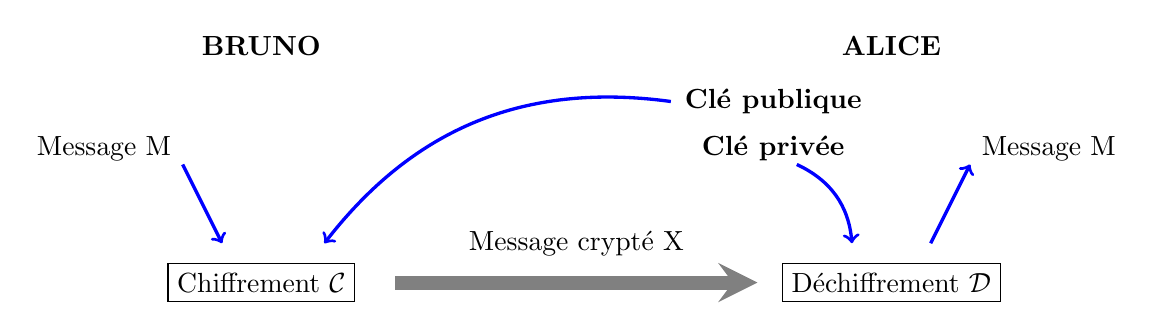
\begin{tikzpicture}

  \node at (4,3) {\bf ALICE};
  \node at (-4,3) {\bf BRUNO};

  \draw[line width=5pt,>=stealth,->,gray] (-2.3,0) to (2.3,0);

  \node at (-6,1.7) {\prive{Message M}};
  \node at (6,1.7) {\prive{Message M}};
  \node at (0,0.5) {\public{Message crypté X}};
  \node at (2.5,2.3) {\bf Clé publique};
  \node at (2.5,1.7) {\bf Clé privée};
  \draw (-4,0)node[draw]{Chiffrement \public{$\mathcal{C}$}};
  \draw (4,0)node[draw]{Déchiffrement \public{$\mathcal{D}$}};

  \draw[->, blue, very thick] (1.2,2.3) to[bend right, thick] (-3.2,0.5);
  \draw[->, blue, very thick] (2.8,1.5) to[bend left, thick] (3.5,0.5);

  \draw[->, blue, very thick] (-5,1.5) to (-4.5,0.5);
  \draw[<-, blue, very thick] (5,1.5) to (4.5,0.5);
\end{tikzpicture}
\end{center}

En prenant appui sur l'exemple précédent, si le message initial est $71$
et que la fonction $f$ de chiffrement est connue de tous,
le message transmis est $11$ et le déchiffrement
sera rapide si la trappe secrète $7$ est connue du destinataire.

Les paramètres d'un protocole de \defi{chiffrement à clé publique} sont donc :
\begin{itemize}
\item les fonctions de chiffrement et de déchiffrement : \public{$\mathcal{C}$} et \public{$\mathcal{D}$},
\item la clé publique du destinataire qui va permettre de paramétrer la fonction \public{$\mathcal{C}$},
\item la clé privée du destinataire qui va permettre de paramétrer la fonction \public{$\mathcal{D}$}.
\end{itemize}
Dans le cadre de notre exemple Bruno souhaite envoyer un message à Alice, ces éléments sont :
\begin{itemize}
\item \public{$\mathcal{C}$} : $x\longmapsto x^? \pmod{100}$ et \public{$\mathcal{D}$} : $x\longmapsto x^? \pmod{100}$,
\item \public{3} : la clé publique d'Alice qui permet de définir complètement la fonction de chiffrement :
$$\public{\mathcal{C}} : x\longmapsto x^\public{3} \pmod{100},$$
\item \prive{7} : la clé privée d'Alice qui permet de définir complètement la fonction de déchiffrement :
$$\prive{\mathcal{D}} : x\longmapsto x^\prive{7} \pmod{100}.$$
\end{itemize}

% Voici une présentation d'un tel protocole. Tout se passe comme si
% Bruno pouvait déposer son message dans la boîte à lettres d'Alice.
% Mais seule Alice possède la clé pour relever le courrier et prendre connaissance du message.
%
% \begin{figure}[htbp]
%     \begin{center}
%       \setlength{\unitlength}{2547sp}%
%       \begin{picture}(5700,2235)(2101,-3961)
%         \thinlines
%         \put(3301,-3961){\makebox(0,0)[cb]{Bruno}}
%         \put(6601,-3961){\makebox(0,0)[cb]{Alice}}
%         \put(3301,-2061){\makebox(0,0)[cb]{\public{Pub(Alice)}}}
%         \put(2101,-3061){\makebox(0,0)[cc]{\prive{$m$}}}
%         \put(3301,-2161){\vector( 0,-1){600}}
%         \put(2401,-3061){\vector( 1, 0){600}}
%         \put(3001,-3361){\framebox(600,600){\public{$C$}}}
%         \put(3601,-3061){\vector( 1, 0){2700}}
%         \put(5001,-2761){\makebox(0,0)[cb]{\public{$c$}}}
%         \put(6601,-2061){\makebox(0,0)[cb]{\prive{Priv(Alice)}}}
%         \put(6301,-3361){\framebox(600,600){\public{$D$}}}
%         \put(6901,-3061){\vector( 1, 0){600}}
%         \put(6601,-2161){\vector( 0,-1){600}}
%         \put(7801,-3061){\makebox(0,0)[cc]{\prive{$m$}}}
%         \put(4600,-3361){\includegraphics[height=1cm]{figures/boite.jpg}}
%       \end{picture}
%     \end{center}
%   \end{figure}



Dans la pratique, un chiffrement à clé publique nécessite plus de calculs et est donc assez lent, plus lent qu'un chiffrement à clé privée. Afin de gagner en rapidité, un protocole hybride peut être mis en place de la façon suivante :
\begin{itemize}
\item à l'aide d'un protocole de chiffrement à clé publique, Alice et Bruno échangent une clé,
\item Alice et Bruno utilise cette clé dans un protocole de chiffrement à clé secrète.
\end{itemize}



%% \begin{figure}[htbp]
%%     \begin{center}
%%       \setlength{\unitlength}{2547sp}%
%%       \begin{picture}(5700,3200)(2101,-3961)
%%         \thinlines
%%         \put(3301,-3961){\makebox(0,0)[cb]{Alice}}
%%         \put(6601,-3961){\makebox(0,0)[cb]{Bruno}}
%%           \put(1501,-1561){\framebox(600,900){}}%message
%%           \put(1651,-800){\line( 1, 0){300}}
%%           \put(1651,-1000){\line( 1, 0){300}}
%%           \put(1651,-1200){\line( 1, 0){300}}
%%           \put(1651,-1400){\line( 1, 0){300}}
%%           \put(7801,-1561){\framebox(600,900){}}%message
%%           \put(7951,-800){\line( 1, 0){300}}
%%           \put(7951,-1000){\line( 1, 0){300}}
%%           \put(7951,-1200){\line( 1, 0){300}}
%%           \put(7951,-1400){\line( 1, 0){300}}
%%           \put(2101,-1161){\vector(1,0){5700}}%horizontal
%%           \put(1801,-1561){\vector(0,-1){1050}}%vertical
%%           \put(1501,-3511){\framebox(600,900){}}%message
%%           \put(1651,-2750){\line( 1, 0){300}}
%%           \put(1651,-2950){\line( 1, 0){300}}
%%           \put(1651,-3150){\line( 1, 0){300}}
%%           \put(1651,-3350){\line( 1, 0){300}}
%%           \put(3301,-2061){\makebox(0,0)[cb]{\prive{Priv(Alice)}}}
%%           \put(3301,-2161){\vector( 0,-1){600}}
%%           \put(2101,-3061){\vector( 1, 0){900}}
%%           \put(3001,-3361){\framebox(600,600){\public{$C$}}}
%%           \put(3601,-3061){\vector( 1, 0){2700}}
%%           \put(5001,-2761){\makebox(0,0)[cb]{\public{$c$}}}
%%           \put(6601,-2061){\makebox(0,0)[cb]{\public{Pub(Alice)}}}
%%           \put(6301,-3361){\framebox(600,600){\public{$D$}}}
%%           \put(6901,-3061){\vector( 1, 0){900}}
%%           \put(6601,-2161){\vector( 0,-1){600}}
%%           \put(7801,-3511){\framebox(600,900){}}%message
%%           \put(7951,-2750){\line( 1, 0){300}}
%%           \put(7951,-2950){\line( 1, 0){300}}
%%           \put(7951,-3150){\line( 1, 0){300}}
%%           \put(7951,-3350){\line( 1, 0){300}}
%%           \put(7801,-1561){\color{blue}{\framebox(600,900){}}}%message
%%           \put(7951,-800){\color{blue}{\line( 1, 0){300}}}
%%           \put(7951,-1000){\color{blue}{\line( 1, 0){300}}}
%%           \put(7951,-1200){\color{blue}{\line( 1, 0){300}}}
%%           \put(7951,-1400){\color{blue}{\line( 1, 0){300}}}
%%           \put(7801,-3511){\color{blue}{\framebox(600,900){}}}%message
%%           \put(7951,-2750){\color{blue}{\line( 1, 0){300}}}
%%           \put(7951,-2950){\color{blue}{\line( 1, 0){300}}}
%%           \put(7951,-3150){\color{blue}{\line( 1, 0){300}}}
%%           \put(7951,-3350){\color{blue}{\line( 1, 0){300}}}
%%           \put(8101,-2086){\color{blue}{\vector(0,1){525}}}%vertical
%%           \put(8101,-2086){\color{blue}{\vector(0,-1){525}}}%vertical
%%         %\visible<10->{\put(4600,-3561){\boite}}
%%       \end{picture}
%%     \end{center}
%%   \end{figure}




%% \begin{figure}[htbp]
%%     \begin{center}
%%       \setlength{\unitlength}{2547sp}%
%%       \begin{picture}(5700,3200)(2101,-3961)
%%         \thinlines
%%         \put(3301,-3961){\makebox(0,0)[cb]{Alice}}
%%         \put(6601,-3961){\makebox(0,0)[cb]{Bruno}}
%%           \put(1501,-1561){\framebox(600,900){}}%message
%%           \put(1651,-800){\line( 1, 0){300}}
%%           \put(1651,-1000){\line( 1, 0){300}}
%%           \put(1651,-1200){\line( 1, 0){300}}
%%           \put(1651,-1400){\line( 1, 0){300}}
%%           \put(7801,-1561){\framebox(600,900){}}%message
%%           \put(7951,-800){\line( 1, 0){300}}
%%           \put(7951,-1000){\line( 1, 0){300}}
%%           \put(7951,-1200){\line( 1, 0){300}}
%%           \put(7951,-1400){\line( 1, 0){300}}
%%           \put(2101,-1161){\vector(1,0){5700}}%horizontal
%%           \put(1501,-3211){{\framebox(600,300){}}}%empreinte
%%           \put(1651,-3061){{\line( 1, 0){300}}}
%%           \put(1400,-2311){\makebox(0,0)[lb]{\public{\small H}}}
%%           \put(1801,-1561){\vector(0,-1){1300}}%vertical
%%           \put(3301,-2061){\makebox(0,0)[cb]{\prive{Priv(Alice)}}}
%%           \put(3301,-2161){\vector( 0,-1){600}}
%%           \put(2101,-3061){\vector( 1, 0){900}}
%%           \put(3001,-3361){\framebox(600,600){\public{$C$}}}
%%           \put(3601,-3061){\vector( 1, 0){2700}}
%%           \put(5001,-2761){\makebox(0,0)[cb]{\public{$c$}}}
%%           \put(6601,-2061){\makebox(0,0)[cb]{\public{Pub(Alice)}}}
%%           \put(6301,-3361){\framebox(600,600){\public{$D$}}}
%%           \put(6901,-3061){\vector( 1, 0){400}}
%%           \put(6601,-2161){\vector( 0,-1){600}}
%%           \put(7301,-3211){{\framebox(600,300){}}}%empreinte
%%           \put(7451,-3061){{\line( 1, 0){300}}}
%%          \put(8601,-1111){{\vector(-1,0){200}}}%vertical
%%           \put(8601,-2086){{\line(0,1){975}}}%vertical
%%           \put(8700,-2086){\makebox(0,0)[lb]{\public{\small H}}}
%%           \put(8601,-2086){{\vector(0,-1){825}}}%vertical
%%           \put(8301,-3211){\framebox(600,300){}}%emprunte
%%           \put(8451,-3061){{\line( 1, 0){300}}}
%%           \put(8101,-3061){\color{blue}{\vector( 1, 0){200}}}
%%           \put(8101,-3061){\color{blue}{\vector( -1, 0){200}}}
%%           \put(8301,-3211){\color{blue}{\framebox(600,300){}}}%emprunte
%%           \put(8451,-3061){\color{blue}{\line( 1, 0){300}}}
%%           \put(7301,-3211){\color{blue}{\framebox(600,300){}}}%empreinte
%%           \put(7451,-3061){\color{blue}{\line( 1, 0){300}}}
%%       \end{picture}
%%     \end{center}
%%   \end{figure}



%  \item Principe sur lequel repose RSA : factorisation de $n=pq$ ;
%  meilleur temps de factorisation connu $\sim e^{(\ln n)^\frac13}$ (c'est moins que $e^n$, mais plus
%  que $n^d$ pour tout $d$, lorsque $n$ tend vers $+\infty$)

%%  \item Signature





%%%%%%%%%%%%%%%%%%%%%%%%%%%%%%%%%%%%%%%%%%%%%%%%%%%%%%%%%%%%%%
\section{L'arithmétique pour RSA}

Pour un entier $n$, sachant qu'il est le produit de deux nombres premiers,
il est difficile de retrouver les facteurs $p$ et $q$ tels que $n=pq$.
Le principe du chiffrement RSA, chiffrement à clé publique, repose sur cette difficulté.

Dans cette partie nous mettons en place les outils mathématiques
nécessaires pour le calcul des clés publique et privée
ainsi que les procédés de chiffrement et déchiffrement RSA.


%-------------------------------------------------------
\subsection{Le petit théorème de Fermat amélioré}

Nous connaissons le petit théorème de Fermat
\begin{theoreme}[Petit théorème de Fermat]
Si $p$ est un nombre premier et $a \in \Zz$ alors
\mybox{$a^p \equiv a \pmod p$}
\end{theoreme}

et sa variante :

\begin{corollaire}
Si $p$ ne divise pas $a$ alors
\mybox{$a^{p-1} \equiv 1 \pmod p$}
\end{corollaire}

Nous allons voir une version améliorée de ce théorème dans le cas qui nous intéresse :

\begin{theoreme}[Petit théorème de Fermat amélioré]
Soient $p$ et $q$ deux nombres premiers distincts et soit $n = p q$. Pour tout
$a\in \Zz$ tel que $\pgcd(a,n)=1$ alors :
\mybox{$a^{(p-1)(q-1)} \equiv 1 \pmod n$}
\end{theoreme}
On note $\varphi(n)=(p-1)(q-1)$, la \defi{fonction d'Euler}.
L'hypothèse $\pgcd(a,n)=1$ équivaut ici à ce que $a$ ne soit divisible ni par $p$, ni par $q$.
Par exemple pour $p=5$, $q=7$, $n=35$ et $\varphi(n)=4\cdot 6 = 24$.
Alors pour $a=1,2,3,4,6,8,9,11,12,13,16,17,18,...$ on a bien $a^{24} \equiv 1 \pmod{35}$.


\begin{proof}
Notons $c = a^{(p-1)(q-1)}$.
Calculons $c$ modulo $p$ :
$$c \equiv a^{(p-1)(q-1)} \equiv (a^{(p-1)})^{q-1} \equiv 1^{q-1} \equiv 1 \pmod{p}$$
où l'on appliquer le petit théorème de Fermat : $a^{p-1} \equiv 1 \pmod p$, car $p$ ne divise pas $a$.

Calculons ce même $c$ mais cette fois modulo $q$ :
$$c \equiv a^{(p-1)(q-1)} \equiv (a^{(q-1)})^{p-1} \equiv 1^{p-1} \equiv 1 \pmod{q}$$
où l'on appliquer le petit théorème de Fermat : $a^{q-1} \equiv 1 \pmod q$, car $q$ ne divise pas $a$.

Conclusion partielle : $c \equiv 1 \pmod{p}$ et $c \equiv 1 \pmod q$.

\bigskip


Nous allons en déduire que $c \equiv 1 \pmod{pq}$.

Comme $c \equiv 1 \pmod{p}$ alors il existe $\alpha \in \Zz$ tel que $c = 1 + \alpha p$ ;
comme $c \equiv 1 \pmod{q}$ alors il existe $\beta \in \Zz$ tel que $c = 1 + \beta q$.
Donc $c-1 = \alpha p = \beta q$.
De l'égalité $\alpha p = \beta q$, on tire que $p | \beta q$.

Comme $p$ et $q$ sont premiers entre eux (car ce sont des nombres premiers distincts)
alors par le lemme de Gauss on en déduit que $p | \beta$.
Il existe donc $\beta'\in \Zz$ tel que $\beta = \beta' p $.

Ainsi $c = 1 + \beta q = 1 + \beta' pq$.
Ce qui fait que $c \equiv 1 \pmod{pq}$,
c'est exactement dire $a^{(p-1)(q-1)} \equiv 1 \pmod n$.
\end{proof}


%-------------------------------------------------------
\subsection{L'algorithme d'Euclide étendu}

Nous avons déjà étudié l'algorithme d'Euclide qui repose sur le principe
que $\pgcd(a,b)= \pgcd(b, a \pmod{b})$.

Voici sa mise en \oe uvre informatique.

\insertcode{algos/euclide-tex1.py}{euclide.py (1)}

On profite que \Python\ assure les affectations simultanées,
ce qui pour nous correspond aux suites
$$\left\{\begin{array}{rcl}
           a_{i+1} & = & b_i \\
           b_{i+1} & \equiv & a_i \pmod {b_i} \\
         \end{array}
 \right.$$
initialisée par $a_0=a$, $b_0=b$.

Nous avons vu aussi comment \og remonter \fg\ l'algorithme d'Euclide à la main pour
obtenir les coefficients de Bézout $u,v$ tels que $au+bv=\pgcd(a,b)$.
Cependant il nous faut une méthode plus automatique pour obtenir ces coefficients, c'est
l'\defi{algorithme d'Euclide étendu}.



On définit deux suites $(x_i)$, $(y_i)$ qui vont aboutir aux coefficients de Bézout.

L'initialisation est :
$$x_0=1 \qquad  x_1=0 \qquad y_0=0 \qquad y_1 = 1$$

et la formule de récurrence pour $i\geq 1$ :
$$x_{i+1} = x_{i-1} - q_i x_i \qquad y_{i+1} = y_{i-1} - q_i y_i$$
 où $q_i$ est le quotient de la division euclidienne de $a_i$ par $b_i$.


\insertcode{algos/euclide-tex2.py}{euclide.py (2)}

Cet algorithme renvoie d'abord le pgcd, puis les coefficients $u,v$ tels que
$au+bv = \pgcd(a,b)$.


%-------------------------------------------------------
\subsection{Inverse modulo $n$}

Soit $a \in \Zz$, on dit que $x \in \Zz$ est un \defi{inverse de $a$ modulo $n$}
si \myboxinline{$ax \equiv 1 \pmod{n}$.}

Trouver un inverse de $a$ modulo $n$ est donc un cas particulier de l'équation $ax \equiv b \pmod n$.

\begin{proposition}
\sauteligne
\begin{itemize}
  \item $a$ admet un inverse modulo $n$ si et seulement si $a$ et $n$ sont premiers entre eux.
  \item Si $au+nv=1$ alors $u$ est un inverse de $a$ modulo $n$.
\end{itemize}
\end{proposition}

En d'autres termes, trouver un inverse de $a$ modulo $n$ revient à calculer les coefficients de Bézout
associés à la paire $(a,n)$.


\begin{proof}
La preuve est essentiellement une reformulation du théorème de Bézout :
$$\begin{array}{rcl}
\pgcd(a,n)=1
       & \iff & \exists u,v \in \Zz \qquad au+nv=1 \\
       & \iff & \exists u \in \Zz \qquad au \equiv 1 \pmod {n} \\
\end{array}$$
\end{proof}

Voici le code :

\insertcode{algos/euclide-tex3.py}{euclide.py (3)}


%-------------------------------------------------------
\subsection{L'exponentiation rapide}

Nous aurons besoin de calculer rapidement des puissances modulo $n$.
Pour cela il existe une méthode beaucoup plus efficace que de calculer d'abord
$a^k$ puis de le réduire modulo $n$. Il faut garder à l'esprit que les entiers
que l'on va manipuler ont des dizaines voire des centaines de chiffres.

Voyons la technique sur l'exemple de $5^{11} \pmod{14}$.
L'idée est de seulement calculer $5, 5^2, 5^4, 5^8...$ %, 5^{16},...$
et de réduire modulo $n$ à chaque fois.
Pour cela on remarque que $11 = 8 + 2 + 1$
donc
$$5 ^{11} = 5^8 \times 5^2 \times 5^1.$$
Calculons donc les $5^{2^i} \pmod {14}$ :
$$
\begin{array}{l}
5  \equiv  5 \pmod{14} \\
5^2  \equiv  25 \equiv 11 \pmod{14} \\
5^4  \equiv 5^2 \times 5^2 \equiv 11 \times 11 \equiv 121 \equiv 9 \pmod{14} \\
5^8  \equiv 5^4 \times 5^4 \equiv 9 \times 9 \equiv 81 \equiv 11 \pmod{14} \\
\end{array}
$$
à chaque étape est effectuée une multiplication modulaire.
Conséquence :
$$5^{11} \equiv 5^8 \times 5^2 \times 5^1 \equiv 11 \times 11 \times 5 \equiv 11 \times 55 \equiv 11 \times 13 \equiv 143 \equiv 3 \pmod{14}.$$
Nous obtenons donc un calcul de $5^{11} \pmod{14}$ en $5$ opérations au lieu de $10$ si on avait fait $5\times 5 \times 5 \cdots$.

Voici une formulation générale de la méthode. On écrit le développement de l'exposant $k$ en base $2$ :
$(k_\ell, \ldots, k_2, k_1, k_0)$ avec $k_i \in \{0,1\}$ de sorte que
$$k = \sum_{i=0}^\ell k_i 2^i.$$
On obtient alors
$$x^k = x^{\sum_{i=0}^\ell k_i 2^i} = \prod_{i=0}^\ell (x^{2^i})^{k_i}.$$

Par exemple $11$ en base $2$ s'écrit $({\color{red}1},{\color{red}0},{\color{red}1},{\color{red}1})$, donc,
comme on l'a vu :
$$5^{11} = (5^{2^3})^{{\color{red}1}} \times (5^{2^2})^{{\color{red}0}}
\times (5^{2^1})^{{\color{red}1}} \times (5^{2^0})^{{\color{red}1}}.$$

Voici un autre exemple : calculons $17^{154} \pmod {100}$.
Tout d'abord on décompose l'exposant $k=154$ en base $2$ :
$154 = 128 + 16 + 8 + 2 = 2^7 + 2^4 + 2^3 + 2^1$, il s'écrit donc en base $2$ : $(1,0,0,1,1,0,1,0)$.

Ensuite on calcule $17, 17^2, 17^4, 17^8,...,17^{128}$ modulo $100$.
$$
\begin{array}{l}
17  \equiv  17 \pmod{100} \\
17^2  \equiv  17 \times 17 \equiv 289 \equiv 89 \pmod{100} \\
17^4  \equiv 17^2 \times 17^2 \equiv 89 \times 89 \equiv 7921 \equiv 21 \pmod{100} \\
17^8  \equiv 17^4 \times 17^4 \equiv 21 \times 21 \equiv 441 \equiv 41 \pmod{100} \\
17^{16}  \equiv 17^8 \times 17^8 \equiv 41 \times 41 \equiv 1681 \equiv 81 \pmod{100} \\
17^{32}  \equiv 17^{16} \times 17^{16} \equiv 81 \times 81 \equiv 6561 \equiv 61 \pmod{100} \\
17^{64}  \equiv 17^{32} \times 17^{32} \equiv 61 \times 61 \equiv 3721 \equiv 21 \pmod{100} \\
17^{128}  \equiv 17^{64} \times 17^{64} \equiv 21 \times 21 \equiv 441 \equiv 41 \pmod{100} \\
\end{array}
$$

Il ne reste qu'à rassembler :
$$17^{154} \equiv 17^{128} \times 17^{16} \times 17^{8} \times 17^{2}
\equiv 41 \times 81 \times 41 \times 89
\equiv 3321 \times 3649
\equiv 21 \times 49
\equiv 1029
\equiv 29 \pmod {100}$$

\bigskip


On en déduit un algorithme pour le calcul rapide des puissances.

\insertcode{algos/puissance-tex.py}{puissance.py}

En fait \Python\ sait faire l'exponentiation rapide :
\codeinline{pow(x,k,n)} pour le calcul de $a^k$ modulo $n$,
il faut donc éviter \codeinline{(x ** k) \% n} qui n'est pas adapté.



%%%%%%%%%%%%%%%%%%%%%%%%%%%%%%%%%%%%%%%%%%%%%%%%%%%%%%%%%%%%%%
\section{Le chiffrement RSA}


Voici le but ultime de ce cours : la chiffrement RSA.
Il est temps de relire l'introduction du chapitre \og Arithmétique \fg\ pour s'apercevoir
que nous sommes prêts !

\bigskip

\begin{center}
\begin{minipage}{0.8\textwidth}
\emph{
Pour crypter un message on commence par le transformer en un --ou plusieurs-- nombres.
Les processus de chiffrement et déchiffrement font appel à plusieurs notions :
\begin{itemize}
  \item On choisit deux \evidence{nombres premiers} $p$ et $q$ que l'on garde secrets et on pose $n=p\times q$.
Le principe étant que même connaissant $n$ il est très difficile de retrouver $p$ et $q$ (qui sont des nombres
ayant des centaines de chiffres).
  \item La clé secrète et la clé publique se calculent à l'aide de l'\evidence{algorithme d'Euclide}
et des \evidence{coefficients de Bézout}.
  \item Les calculs de cryptage se feront \evidence{modulo} $n$.
  \item Le déchiffrement fonctionne grâce à une variante du \evidence{petit théorème de Fermat}.
\end{itemize}
}
\end{minipage}
\end{center}


\bigskip



Dans cette section, c'est Bruno qui veut envoyer un message secret à Alice.
La processus se décompose ainsi :
\begin{enumerate}
  \item Alice prépare une clé publique et une clé privée,
  \item Bruno utilise la clé publique d'Alice pour crypter son message,
  \item Alice reçoit le message crypté et le déchiffre grâce à sa clé privée.
\end{enumerate}




%-------------------------------------------------------
\subsection{Calcul de la clé publique et de la clé privée}

%.......................................................
\subsubsection{Choix de deux nombres premiers}

Alice effectue, une fois pour toute, les opérations suivantes (en secret) :
\begin{itemize}
  \item elle choisit deux nombres premiers distincts $\prive{p}$ et $\prive{q}$ (dans la pratique ce sont de très grand nombres,
  jusqu'à des centaines de chiffres),

  \item Elle calcule $\public{n} = \prive{p} \times \prive{q}$,

  \item Elle calcule $\varphi(\public{n}) = (\prive{p}-1) \times (\prive{q}-1)$.
\end{itemize}

\bigskip

\textbf{Exemple 1.}
 \begin{itemize}
  \item $\prive{p} = 5$ et $\prive{q} = 17$

  \item $\public{n} = \prive{p} \times \prive{q} = 85$

  \item $\prive{\varphi(n)} = (\prive{p}-1) \times (\prive{q}-1) = 64$
\end{itemize}

Vous noterez que le calcul de $\prive{\varphi(n)}$ n'est possible que
si la décomposition de $\public{n}$ sous la forme $\prive{p}\times \prive{q}$ est connue.
D'où le caractère secret de $\prive{\varphi(n)}$ même si $\public{n}$ est connu de tous.

\bigskip

\textbf{Exemple 2.}
 \begin{itemize}
  \item $\prive{p} = 101$ et $\prive{q} = 103$

  \item $\public{n} = \prive{p} \times \prive{q} = 10\;403$

  \item $\prive{\varphi(n)} = (\prive{p}-1) \times (\prive{q}-1) = 10\;200$
\end{itemize}

%.......................................................
\subsubsection{Choix d'un exposant et calcul de son inverse}

Alice continue :
\begin{itemize}
  \item elle choisit un exposant $\public{e}$ tel que $\pgcd(\public{e},\prive{\varphi(n)})=1$,

  \item elle calcule l'inverse $\prive{d}$ de $\public{e}$ module $\prive{\varphi(n)}$ :
  $\prive{d} \times \public{e} \equiv 1 \pmod {\prive{\varphi(n)}}$.
  Ce calcul se fait par l'algorithme d'Euclide étendu.
\end{itemize}

\bigskip

\textbf{Exemple 1.}
\begin{itemize}
  \item Alice choisit par exemple $\public{e} = 5$ et on a bien  $\pgcd(\public{e},\prive{\varphi(n)}) = \pgcd(5,64)=1$,

  \item Alice applique l'algorithme d'Euclide étendu pour calculer les coefficients de Bézout correspondant à
  $\pgcd(\public{e},\prive{\varphi(n)})=1$. Elle trouve
  $5 \times 13 + 64 \times (-1) = 1$. Donc $5 \times 13 \equiv 1 \pmod {64}$
  et l'inverse de $\public{e}$ modulo $\prive{\varphi(n)}$ est $\prive{d} = 13$.

\end{itemize}

\bigskip

\textbf{Exemple 2.}
\begin{itemize}
  \item Alice choisit par exemple $\public{e} = 7$ et on a bien  $\pgcd(\public{e},\prive{\varphi(n)}) = \pgcd(7,10\;200)=1$,

  \item L'algorithme d'Euclide étendu pour $\pgcd(\public{e},\prive{\varphi(n)})=1$ donne
  $7 \times (-1457) + 10\; 200 \times 1 = 1$. Mais $-1457 \equiv 8743\pmod{\prive{\varphi(n)}}$,
  donc pour $\prive{d} = 8743 $
  on a   $\prive{d} \times \public{e} \equiv 1 \pmod {\prive{\varphi(n)}}$.
\end{itemize}

%.......................................................
\subsubsection{Clé publique}

La \defi{clé publique} d'Alice est constituée des deux nombres :
\mybox{$\public{n}$ \  et \  $\public{e}$}

Et comme son nom l'indique Alice communique sa clé publique au monde entier.

\bigskip

\textbf{Exemple 1.} $\public{n} = 85$ et $\public{e} = 5$

\bigskip

\textbf{Exemple 2.} $\public{n} = 10\;403$ et $\public{e} = 7$

%.......................................................
\subsubsection{Clé privée}

Alice garde pour elle sa \defi{clé privée} :
\mybox{\ $\prive{d}$\ }

Alice détruit en secret $\prive{p}$, $\prive{q}$ et $\prive{\varphi(n)}$ qui ne sont plus utiles.
Elle conserve secrètement sa clé privée.


\bigskip

\textbf{Exemple 1.} $\prive{d} = 13$

\bigskip

\textbf{Exemple 2.} $\prive{d} = 8743$


%-------------------------------------------------------
\subsection{Chiffrement du message}


Bruno veut envoyer un message secret à Alice.
Il se débrouille pour que son message soit un entier
(quitte à découper son texte en bloc et à transformer chaque bloc en un entier).



%.......................................................
\subsubsection{Message}

Le message est un entier $\prive{m}$, tel que $0 \le \prive{m} < \public{n}$.

\bigskip

\textbf{Exemple 1.} Bruno veut envoyer le message $\prive{m}=10$.

\bigskip

\textbf{Exemple 2.} Bruno veut envoyer le message $\prive{m}=1234$.

%.......................................................
\subsubsection{Message chiffré}

Bruno récupère la clé publique d'Alice : $\public{n}$ et $\public{e}$
avec laquelle il calcule, à l'aide de l'algorithme d'exponentiation rapide, le message chiffré :
\mybox{$\public{x} \equiv \prive{m}^\public{e} \pmod{\public{n}}$}

Il transmet ce message $\public{x}$ à Alice

\bigskip

\textbf{Exemple 1.} $\prive{m} = 10$, $\public{n} = 85$ et $\public{e} = 5$
donc
$$\public{x} \equiv \prive{m}^\public{e} \pmod {\public{n}} \equiv 10^{5} \pmod {85}$$

On peut ici faire les calculs à la main :
$$\begin{array}{l}
10^2 \equiv 100 \equiv 15 \pmod {85} \\
10^4 \equiv (10^2)^2 \equiv 15^2 \equiv 225 \equiv 55 \pmod{85} \\
\public{x} \equiv 10^5 \equiv 10^4 \times 10 \equiv 55 \times 10 \equiv 550 \equiv 40 \pmod{85}\\
\end{array}$$

Le message chiffré est donc $\public{x}=40$.

\bigskip

\textbf{Exemple 2.} $\prive{m} = 1234$, $\public{n} = 10\;403$ et $\public{e} = 7$
donc
$$\public{x} \equiv \prive{m}^\public{e} \pmod {\public{n}} \equiv 1234^{7} \pmod {10\;403}$$

On utilise l'ordinateur pour obtenir que $\public{x}= 10 \; 378$.

%-------------------------------------------------------
\subsection{Déchiffrement du message}

Alice reçoit le message $\public{x}$ chiffré par Bruno, elle le décrypte à l'aide de sa clé privée $\prive{d}$,
par l'opération :

\mybox{$\prive{m} \equiv \public{x}^\prive{d} \pmod {\public{n}}$}
qui utilise également l'algorithme d'exponentiation rapide.

Nous allons prouver dans le lemme \ref{lem:dechiffre}, que par cette opération
Alice retrouve bien le message original $\prive{m}$ de Bruno.

\bigskip

\textbf{Exemple 1.} $\prive{c} = 40$, $\prive{d} = 13$, $\public{n} = 85$
donc
$$\public{x}^\prive{d} \equiv (40)^{13} \pmod{85}.$$

Calculons à la main
$40^{13} \equiv \pmod {85}$ on note que $13 = 8 + 4 + 1$,
donc $40^{13} = 40^8 \times 40^4 \times 40$.

$$\begin{array}{l}
  40^2 \equiv 1600 \equiv 70 \pmod{85} \\
  40^4 \equiv (40^2)^2 \equiv 70^2 \equiv 4900 \equiv 55 \pmod{85} \\
  40^8 \equiv (40^4)^2 \equiv 55^2 \equiv 3025 \equiv 50 \pmod{85} \\
\end{array}$$
Donc
$$\public{x}^\prive{d} \equiv 40^{13} \equiv 40^8 \times 40^4 \times 40 \equiv 50 \times 55 \times 40 \equiv 10 \pmod{85}$$
qui est bien le message $\prive{m}$ de Bruno.

\bigskip

\textbf{Exemple 2.} $\prive{c} = 10 \; 378$, $\prive{d} = 8743$, $\public{n} = 10\;403$.
On calcule par ordinateur $\public{x}^\prive{d} \equiv (10 \; 378)^{8743} \pmod{10\;403}$
qui vaut exactement le message original de Bruno $\prive{m}=1234$.

%-------------------------------------------------------
\subsection{Schéma}

\begin{figure}[htbp]
    \begin{center}
      \setlength{\unitlength}{2547sp}%
      \begin{picture}(7000,2235)(2101,-3961)
        \thinlines
        \put(3301,-3961){\makebox(0,0)[cb]{Bruno}}
        \put(6601,-3961){\makebox(0,0)[cb]{Alice}}
        \put(3301,-2061){\makebox(0,0)[cb]{\public{$n$}, \public{$e$}}}
        \put(2101,-3061){\makebox(0,0)[cc]{\prive{$m$}}}
        \put(3301,-2161){\vector( 0,-1){600}}
        \put(2401,-3061){\vector( 1, 0){600}}
        \put(3001,-3361){\framebox(600,600){\public{$\mathcal{C}$}}}
        \put(3601,-3061){\vector( 1, 0){2700}}
        \put(5001,-2761){\makebox(0,0)[cb]{$\public{x} \equiv \prive{m}^\public{e} \pmod {\public{n}} $}}
        \put(6601,-2061){\makebox(0,0)[cb]{\prive{$d$}}}
        \put(6301,-3361){\framebox(600,600){\public{$\mathcal{D}$}}}
        \put(6901,-3061){\vector( 1, 0){600}}
        \put(6601,-2161){\vector( 0,-1){600}}
        \put(7801,-3061){\makebox(0,0)[lc]{$\prive{m} \equiv \public{x}^\prive{d} \pmod{\public{n}}$}}
%        \put(4600,-3361){\includegraphics[height=1cm]{figures/boite.jpg}}
      \end{picture}
    \end{center}
  \end{figure}

~


Clés d'Alice :
\begin{itemize}
\item publique : \public{$n$}, \public{$e$}
\item privée : \prive{$d$}
\end{itemize}

%-------------------------------------------------------
\subsection{Lemme de déchiffrement}

Le principe de déchiffrement repose sur le petit théorème de Fermat amélioré.

\begin{lemme}
\label{lem:dechiffre}
Soit $d$ l'inverse de $e$ modulo $\varphi(n)$.
\mybox{Si $x \equiv m^e \pmod n$ alors $m \equiv x^d \pmod n$.}
\end{lemme}

Ce lemme prouve bien que le message original $\prive{m}$ de Bruno,
chiffré par clé publique d'Alice $(\public{e},\public{n})$ en le message $\public{x}$,
peut-être retrouvé par Alice à l'aide de sa clé secrète $\prive{d}$.

\begin{proof}
\begin{itemize}
  \item Que $d$ soit l'inverse de $e$ modulo $\varphi(n)$ signifie
$d \cdot e \equiv 1 \pmod {\varphi(n)}$.
Autrement dit, il existe
$k \in \Zz$ tel que $d \cdot e = 1 + k \cdot \varphi(n)$.

  \item On rappelle que par le petit théorème de Fermat généralisé :
  lorsque $m$ et $n$ sont premiers entre eux
  $$m^{\varphi(n)} \equiv m^{(p-1)(q-1)} \equiv 1 \pmod n$$


  \item \textbf{Premier cas} $\pgcd(m,n)=1$.

  Notons $c \equiv m^e \pmod n$ et calculons $x^d$ :

$$x^d \equiv (m^e)^d
      \equiv m^{e\cdot d}
      \equiv m^{1+k \cdot \varphi(n)}
      \equiv m \cdot m^{k \cdot \varphi(n)}
      \equiv m \cdot (m^{\varphi(n)})^k
      \equiv m \cdot (1)^k
      \equiv m \pmod {n}$$

 \item \textbf{Deuxième cas} $\pgcd(m,n) \neq 1$.

Comme $n$ est le produit des deux nombres premiers $p$ et $q$ et que $m$
est strictement plus petit que $n$ alors si $m$ et $n$ ne sont pas premiers entre eux cela implique que
$p$ divise $m$ ou bien $q$ divise $m$ (mais pas les deux en même temps).
Faisons l'hypothèse $\pgcd(m,n)=p$ et  $\pgcd(m,q)=1$,
le cas  $\pgcd(m,n)=q$  et $\pgcd(m,p)=1$ se traiterait de la même manière.

\'Etudions $(m^e)^d$ à la fois modulo $p$ et modulo $q$
à l'image de ce que nous avons fait dans la preuve du théorème de Fermat amélioré.
\begin{itemize}
\item modulo $p$ : $m   \equiv  0 \pmod{p}$  et $(m^e)^d \equiv  0 \pmod{p}$
donc  $(m^e)^d \equiv  m   \pmod{p}$,

\item modulo $q$ : $(m^e)^d  \equiv m \!\times\! (m^{\varphi(n)})^k \equiv m \!\times\! (m^{q-1})^{(p-1)k}
\equiv m   \pmod{q}$.
\end{itemize}
Comme $p$ et $q$ sont deux nombres premiers distincts, ils sont premiers entre eux
et on peut écrire comme dans la preuve du petit théorème de Fermat amélioré que
$$(m^e)^d  \equiv  m \pmod{n}$$
\end{itemize}

\end{proof}


%-------------------------------------------------------
\subsection{Algorithmes}

La mise en \oe uvre est maintenant très simple. Alice choisit
deux nombres premiers $\prive{p}$ et $\prive{q}$ et un exposant $\public{e}$.

Voici le calcul de la clé secrète :
\insertcode{algos/rsa-tex1.py}{rsa.py (1)}


Le chiffrement d'un message \prive{$m$} est possible par tout le monde,
connaissant la clé publique $(\public{n},\public{e})$.

\insertcode{algos/rsa-tex2.py}{rsa.py (2)}

Seule Alice peut déchiffrer le message crypté $\public{x}$, à l'aide de sa clé privée $\prive{d}$.

\insertcode{algos/rsa-tex3.py}{rsa.py (3)}


%%%%%%%%%%%%%%%%%%%%%%%%%%%%%%%%%%%%%%%%%%%%%%%%%%%%%%%%%%%%%%%%
\section*{Pour continuer...}


Bibliographie commentée :

\begin{enumerate}


  \item \textbf{Histoire des codes secrets} de Simon Singh, Le livre de Poche.

  Les codes secrets racontés comme un roman policier. Passionnant.
  Idéal pour les plus littéraires.


  \item \textbf{Comprendre les codes secrets} de Pierre Vigoureux, édition Ellipses.

  Un petit livre très clair et très bien écrit, qui présente un panorama complet
  de la cryptographie sans rentrer dans les détails mathématiques. Idéal pour les
  esprits logiques.


  \item \textbf{Codage et cryptographie} de Joan G\'omez, édition Le Monde -- Images des mathématiques.
  Un autre petit livre très clair et très bien, un peu de maths, des explications claires et
  des encarts historiques intéressants.


  \item \textbf{Introduction à la cryptographie} de Johannes Buchmann, édition Dunod.

  Un livre d'un niveau avancé (troisième année de licence) pour comprendre les méthodes
  mathématiques de la cryptographie moderne.  Idéal pour unifier les points de vue des
  mathématiques avec l'informatique.

%   \item \textbf{Cours de cryptographie} de Gilles Zémor, édition Cassini.
%
%   Un livre très mathématique (troisième année de licence).

  \item \textbf{Algèbre - Première année} de Liret et Martinais, édition Dunod.

  Livre qui recouvre tout le programme d'algèbre de la première année, très bien adapté aux étudiants des l'université.
  Pas de cryptographie.
\end{enumerate}


\auteurs{
Arnaud Bodin, 
François Recher
}

\finchapitre
\end{document}

